% Chapter 5: Response Surface Analysis (RSM Analysis page and Coefficient Table page)
\chapter{Response Surface Analysis}\label{sec:ch05-rsm}\label{chap:5}

The \ui{RSM Analysis} page (navigation group \ui{Analysis}) is where a regression model is chosen,
fitted and checked for each response. Everything that the later pages use (model graphs, desirability,
NSGA-II, sensitivity, prediction) is built on the model that is selected here, unless the response is
switched to an ANN model on the \ui{ANN} page. This chapter describes the page from top to bottom: the
toolbars, the term list and the six sub-tabs \ui{Fit Summary}, \ui{ANOVA}, \ui{Model Equation},
\ui{Diagnostics}, \ui{Box-Cox} and \ui{Effects (Factorial)}. It also covers the two special analyses that
replace ordinary least squares for some responses (logistic and Poisson regression, and the split-plot
REML analysis) and the \ui{Coefficient Table} page, which shows the coefficients of all responses side by
side.

The numbers in the examples come from the built-in case studies (\menupath{File $\rightarrow$ Case
Studies}). The case studies use fixed data, so you can reproduce every value.

\section{The RSM Analysis page at a glance}\label{sec:ch05-page}

\subsection*{Purpose}
The page answers three questions for one response at a time: which polynomial model describes the data
adequately, which terms of that model are needed, and whether the assumptions behind the statistical tests
are met.

\subsection*{How to use (typical workflow)}
\begin{enumerate}
  \item Select the response in \ui{Response:}.
  \item Read the \ui{Fit Summary} sub-tab and click \ui{Use Suggested Model} (or choose an order in
        \ui{Model:} yourself).
  \item Read the \ui{ANOVA} sub-tab: model significance, term p-values, lack of fit and the fit
        statistics.
  \item Remove terms that are not needed, either by unchecking them in the term list or with
        \ui{Backward Elimination}.
  \item Check the residuals on the \ui{Diagnostics} sub-tab and, if needed, the \ui{Box-Cox} sub-tab.
        Apply a transformation or exclude a faulty run, then go back to step 2.
  \item Read the final equation on the \ui{Model Equation} sub-tab.
  \item Repeat for the other responses and compare them on the \ui{Coefficient Table} page.
\end{enumerate}
Every change (order, terms, transformation, excluded runs) is stored in the project and immediately used
by the \ui{Coefficient Table}, \ui{Model Graphs}, optimization and prediction pages.

\begin{figure}[htbp]\centering
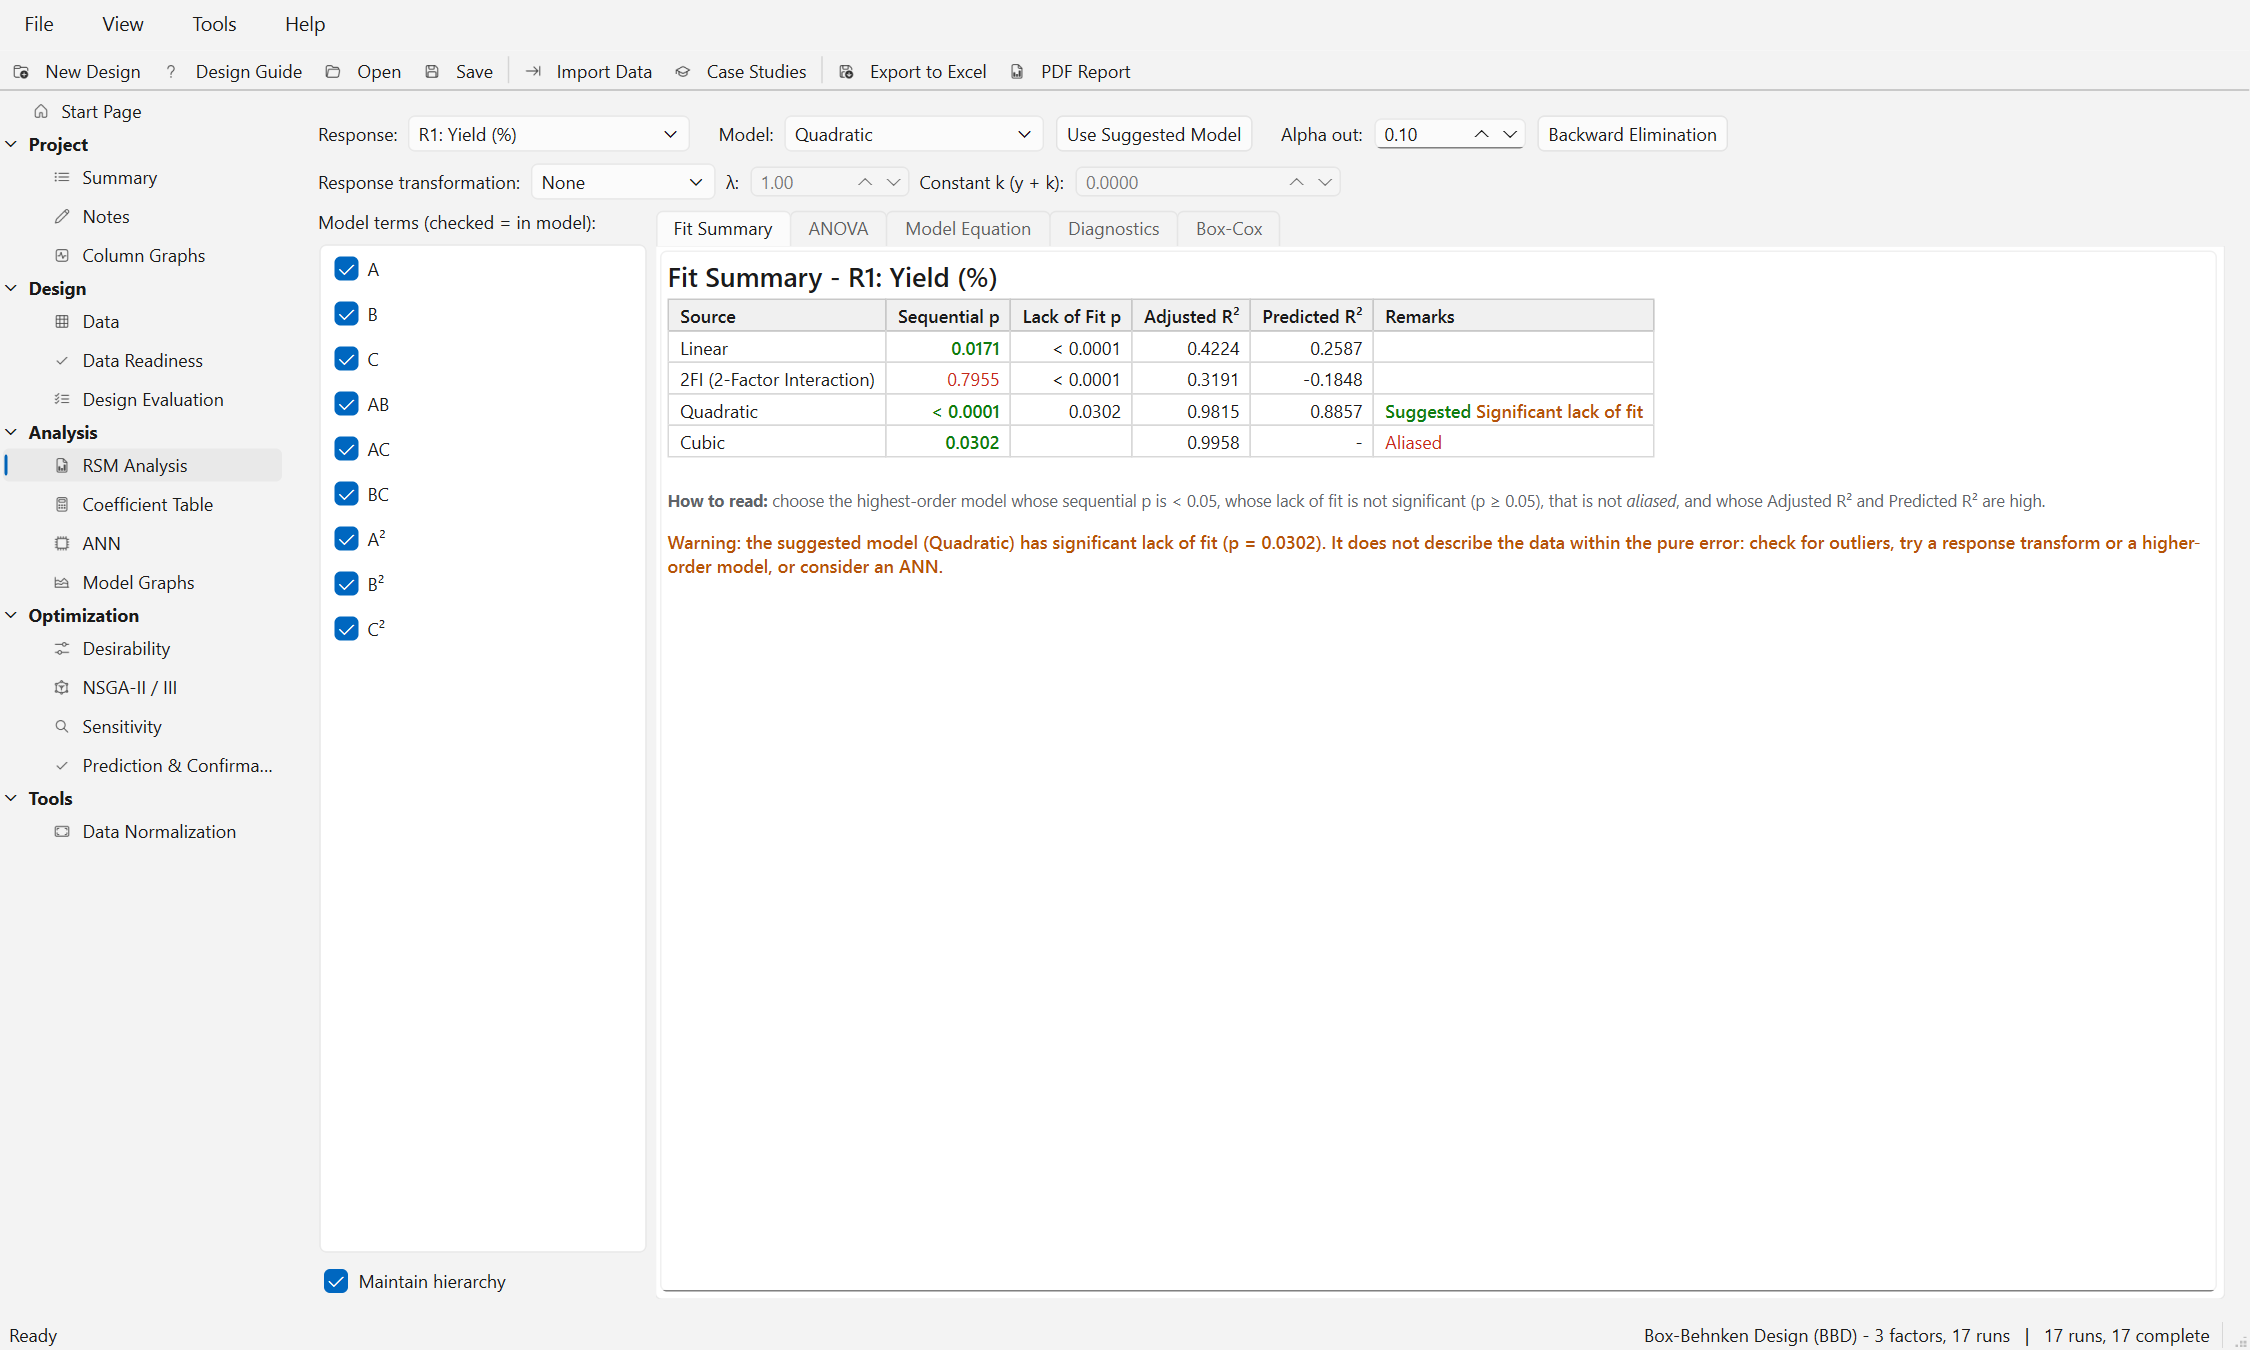
\includegraphics[width=\linewidth]{rsm_fit_summary.png}
\caption{RSM Analysis page, \ui{Fit Summary} sub-tab, for the response Yield of the Box-Behnken extraction
case. Top: the two toolbar rows. Left: the term list with \ui{Maintain hierarchy}. Right: the sequential
model table with the suggested model (Quadratic, remark \ui{Significant lack of fit}) and, below the note, the
lack-of-fit warning (p = 0.0302).}
\label{fig:ch05-fitsummary}
\end{figure}

\subsection*{Toolbar controls}
Table~\ref{tab:ch05-toolbar} lists the controls of the two toolbar rows above the sub-tabs
(Figure~\ref{fig:ch05-fitsummary}).

\begin{table}[htbp]\centering\small
\caption{Toolbar controls of the RSM Analysis page.}\label{tab:ch05-toolbar}
\begin{tabularx}{\linewidth}{@{}>{\raggedright\arraybackslash}p{3.0cm} >{\raggedright\arraybackslash}p{3.6cm} >{\raggedright\arraybackslash}p{1.6cm} X@{}}
\toprule
Control & Values & Default & Meaning \\
\midrule
\ui{Response:} & each response, e.g.\ \ui{R1: Yield (\%)} & first response & Response whose model is shown and edited. \\
\ui{Model:} & orders valid for the design (Table~\ref{tab:ch05-orders}) & design dependent & Model order. Changing it resets the term list to the full set of terms of that order. \\
\ui{Use Suggested Model} & button & -- & Switches \ui{Model:} to the order marked \emph{Suggested} in the Fit Summary. Disabled when nothing beats the mean; hidden for split-plot (REML) responses. \\
\ui{Alpha out:} & 0.01--0.50, step 0.01 & 0.10 & Significance level used by backward elimination. \\
\ui{Backward Elimination} & button & -- & Removes non-significant terms one at a time (Section~\ref{sec:ch05-backward}). \\
\ui{Response transformation:} & None, Square root, Natural log (ln), Base 10 log, Inverse (1/y), Power (y\^{}$\lambda$) & None & Transformation of the response before fitting (Section~\ref{sec:ch05-transform}). Disabled for binomial and Poisson responses. \\
\ui{$\lambda$:} & $-3$ to 3, step 0.1 & 1.00 & Exponent of the power transformation; enabled only for \ui{Power}. \\
\ui{Constant k (y + k):} & any number, 4 decimals & 0 & Constant added before the transformation; enabled when a transformation is selected. \\
\bottomrule
\end{tabularx}
\end{table}

A red text to the right of the second toolbar row shows errors of the current fit, for example
``The Natural log (ln) transform requires all response values $>$ 0.'' The message about too few data
is not repeated there; it appears in the sub-tabs instead.

\subsection*{Messages before a model exists}
With fewer than three complete rows (all factors and the response filled in), every report sub-tab shows
``The model cannot be computed yet'' followed by ``Fill in at least 3 complete rows (factors + response) to
start the analysis.'' If the model has no residual degrees of freedom, the ANOVA sub-tab shows
``Residual degrees of freedom = 0 (saturated model). Statistical tests cannot be computed - remove model
terms or add runs.'' The coefficients and the equation are still shown in that case.

\section{Model orders and term selection}\label{sec:ch05-terms}

\subsection*{Purpose}
The model order defines the candidate polynomial; the term list decides which of its terms are actually in
the model.

\subsection*{Model orders}
The orders offered in \ui{Model:} depend on the design type (Table~\ref{tab:ch05-orders}). Orders that give
exactly the same set of terms as an earlier order are not listed (for example, with a single process
factor, \emph{2FI} gives the same process terms as \emph{Linear}).

\begin{table}[htbp]\centering\small
\caption{Model orders offered for each design type and the default order.}\label{tab:ch05-orders}
\begin{tabularx}{\linewidth}{@{}X X l@{}}
\toprule
Design type & Orders offered & Default \\
\midrule
Full, fractional and general factorial & Linear, 2FI, 3FI & 2FI \\
Plackett-Burman & Linear, 2FI, 3FI & Linear \\
Definitive screening, Taguchi & Linear, 2FI, Quadratic, Cubic & Linear \\
CCD, Box-Behnken, optimal (process), historical, space-filling & Linear, 2FI, Quadratic, Cubic & Quadratic \\
Mixture (simplex lattice, simplex centroid, optimal, historical mixture) & Linear, Quadratic, Special Cubic, Cubic & Quadratic \\
Combined mixture-process & Linear $\times$ Mean, Linear $\times$ Linear, Linear $\times$ 2FI, Quadratic $\times$ Linear, Quadratic $\times$ 2FI, Quadratic $\times$ Quadratic, Special Cubic $\times$ Linear, Special Cubic $\times$ 2FI & Quadratic $\times$ Linear \\
\bottomrule
\end{tabularx}
\end{table}

For process factors a term is written as a vector of exponents $(e_1,\dots,e_k)$ and the model of order
$d$ contains every term with $\sum_i e_i\le d$:
\begin{itemize}
  \item \emph{Linear}: $d=1$; \emph{2FI}: $d=2$ and every $e_i\le 1$; \emph{3FI}: $d=3$ and every
        $e_i\le1$ (no squares);
  \item \emph{Quadratic}: $d=2$ (squares allowed); \emph{Cubic}: $d=3$ (squares and cubes allowed);
  \item a categoric factor never gets an exponent above 1.
\end{itemize}
Terms are named with factor letters (\ui{A}, \ui{AB}, \ui{A²}) and listed by total degree, then by the
largest exponent. A project created with a planned model (for example an optimal design) starts with
that order.

\subsection*{How to use the term list}
\begin{enumerate}
  \item The list \ui{Model terms (checked = in model):} shows all terms of the selected order (the
        intercept is not listed; it is always in the model, except in Scheffé mixture models). Terms that
        were added earlier and are not part of the order are listed at the end.
  \item Uncheck a term to remove it; check it to put it back. The fit is updated at once.
  \item In mixture designs the linear blending terms (\ui{A}, \ui{B}, \ui{C}, \dots) are greyed out:
        they are always in a Scheffé model.
\end{enumerate}

\subsection*{Maintain hierarchy}
The check box \ui{Maintain hierarchy} below the list (checked by default) keeps the model hierarchical:
\begin{itemize}
  \item checking a term also checks its parent terms (checking \ui{AB} checks \ui{A} and \ui{B};
        checking \ui{A²} checks \ui{A});
  \item unchecking a term also unchecks every term that contains it (unchecking \ui{A} removes \ui{AB},
        \ui{A²}, \ui{ABC}, \dots);
  \item turning the option on adds the missing parent terms of the current model.
\end{itemize}
A term $t$ is a parent of term $u$ when every exponent of $t$ is at most the corresponding exponent of $u$.
For the full cubic mixture term $x_ix_j(x_i-x_j)$ the exponents of $x_i^2x_j$ are used. The same option
applies to clicks on the effects plot (Section~\ref{sec:ch05-effects}) and to \ui{Backward Elimination}
(Section~\ref{sec:ch05-backward}). With the option off, any subset of
terms can be fitted. A hierarchical model is recommended because a non-hierarchical model changes when the
factors are recoded (for example from coded to actual units) \citep{montgomery2017,myers2016}.

\subsection*{Aliased terms}
A term that cannot be estimated from the data (its column is a linear combination of the columns before
it) is removed automatically and listed on the ANOVA sub-tab as ``Aliased terms (removed automatically):
\dots''. The check is done on the columns in the order intercept, blocks, terms. A column is kept only if
it raises the rank of the kept columns; the rank uses the $R$ factor of a QR decomposition with the
tolerance $10^{-8}\cdot\max(1,\max|X|)\cdot\max(n,\text{columns})$.

\section{Coding of factors}\label{sec:ch05-coding}

All models are fitted in coded units. The coding depends on the kind of factor.

\paragraph{Numeric process factors.} A factor with range $[\text{low},\text{high}]$ is coded as
\begin{equation}
  z=\frac{x-c}{h},\qquad c=\frac{\text{low}+\text{high}}{2},\qquad h=\frac{\text{high}-\text{low}}{2},
  \label{eq:ch05-coding}
\end{equation}
so the low level is $-1$ and the high level $+1$. Axial points of a CCD lie outside $[-1,1]$.

\paragraph{Categoric factors (effect coding).} A categoric factor with $L$ levels is expanded into $L-1$
columns. In column $j$ ($j=1,\dots,L-1$)
\begin{equation}
  d_j=\begin{cases}1 & \text{level } j,\\ -1 & \text{last level } L,\\ 0 & \text{otherwise.}\end{cases}
  \label{eq:ch05-effectcode}
\end{equation}
The coefficient of \ui{C[level]} is the difference between that level and the mean over all levels; the
implied coefficient of the last level is minus the sum of the others. Interactions with a categoric factor
are products of the numeric part with each effect-coded column, so \ui{AC} has $L-1$ columns and $L-1$
degrees of freedom. The ANOVA sub-tab repeats this rule in a note.

\paragraph{Blocks.} Blocks are coded with sum-to-zero columns ($b-1$ columns, the last block $-1$). The
block effect is removed first and not tested (note: ``The block effect is removed first and is not
tested.''). Predictions set the block columns to zero, so they refer to the average over the blocks.

\paragraph{Mixture components.} Components are converted to pseudo-components
\begin{equation}
  z_i=\frac{x_i-L_i}{T-\sum_j L_j},
  \label{eq:ch05-pseudo}
\end{equation}
where $T$ is the mixture total and $L_i$ the lower limits. The pseudo-components lie in $[0,1]$ and sum to 1.

\paragraph{Scheffé models.} Mixture models have no intercept, because $\sum z_i=1$ makes it redundant
\citep{scheffe1958,cornell2002}:
\begin{align}
  \text{Linear:}\quad &\hat y=\sum_i\beta_i z_i, \label{eq:ch05-scheffe-lin}\\
  \text{Quadratic:}\quad &\hat y=\sum_i\beta_i z_i+\sum_{i<j}\beta_{ij}z_iz_j, \label{eq:ch05-scheffe-quad}\\
  \text{Special cubic:}\quad &\text{quadratic}+\sum_{i<j<k}\beta_{ijk}z_iz_jz_k, \label{eq:ch05-scheffe-sc}\\
  \text{Cubic:}\quad &\text{special cubic}+\sum_{i<j}\delta_{ij}z_iz_j(z_i-z_j). \label{eq:ch05-scheffe-cub}
\end{align}
The full cubic terms are named \ui{AB(A-B)}. The linear coefficients $\beta_i$ are the predicted responses
of the pure pseudo-component blends (the vertices).

\paragraph{Combined mixture-process models.} Each Scheffé term of the mixture order (without the full
cubic terms) is multiplied by each term of the process order, including the process intercept. With three
components and one process factor $D$, \emph{Quadratic $\times$ Linear} has the 12 terms A, B, C, AB, AC,
BC, AD, BD, CD, ABD, ACD, BCD.

\paragraph{Example (categoric factor).} In the case study \emph{Extraction with Solvent Type (Categoric)}
(CCD, 33 runs, Solvent = Ethanol, Methanol, Acetone), the quadratic model has the coefficients
C[Ethanol] = 0.24848 and C[Methanol] = 2.7694. The implied Acetone effect is
$-(0.24848+2.7694)=-3.018$: Methanol gives about 2.8 percentage points more yield than the average solvent,
Acetone about 3.0 points less. In the ANOVA the term C has 2 df ($F=481.0$) and AC has 2 df ($p=0.0001$).

\section{Least-squares fit (theory as implemented)}\label{sec:ch05-ols}

For a response with $n$ usable runs (rows with a response value and complete factor settings, minus
excluded runs) the model matrix $X$ has $p$ columns after aliased columns are removed (intercept and block
columns included). The response is first transformed (Section~\ref{sec:ch05-transform}). Then
\begin{align}
  \hat\beta&=(X'X)^{+}X'y, &
  e&=y-X\hat\beta, &
  \text{MSE}&=\frac{\text{SSE}}{n-p},\label{eq:ch05-ols}\\
  \text{se}(\hat\beta_j)&=\sqrt{\text{MSE}\,[(X'X)^{+}]_{jj}}, &
  h_{ii}&=x_i'(X'X)^{+}x_i, &
  \text{VIF}_j&=[(X'X)^{+}]_{jj}\sum_i(x_{ij}-\bar x_j)^2,\label{eq:ch05-se}
\end{align}
where $(\cdot)^{+}$ is the pseudo-inverse, $h_{ii}$ the leverage and VIF the variance inflation factor.
VIF is not computed for intercept-free mixture models (the cell is blank). For data sets with more than
400 runs the partial sums of squares are computed from the cross-product matrix $X'X$ instead of
refitting with all rows; the result is the same and the computation does not grow with $n$.

\section{Fit Summary}\label{sec:ch05-fitsummary}

\subsection*{Purpose}
The Fit Summary compares the model orders of Table~\ref{tab:ch05-orders} with sequential tests and suggests
the highest order that adds significant information and can be estimated.

\subsection*{How to use}
\begin{enumerate}
  \item Open the \ui{Fit Summary} sub-tab; it is computed for the full term set of every order.
  \item Read the table from top to bottom. The row marked \ui{Suggested} is the suggestion.
  \item Click \ui{Use Suggested Model} to select it, or choose another order in \ui{Model:}.
\end{enumerate}

\subsection*{Output and how to read it}
The table has the columns \ui{Source}, \ui{Sequential p}, \ui{Lack of Fit p}, \ui{Adjusted R²},
\ui{Predicted R²} and \ui{Remarks}. \ui{Sequential p} is green when $p<0.05$. Remarks are \ui{Suggested},
\ui{Significant lack of fit} (added to the suggested order when its lack-of-fit $p<0.05$) and \ui{Aliased} (the
order contains terms that cannot be estimated). A dash means that the value cannot be
computed (for example Predicted R² when a run has leverage 1). The note below the table reads:
``How to read: choose the highest-order model whose sequential p is $<$ 0.05, whose lack of fit is not
significant (p $\ge$ 0.05), that is not aliased, and whose Adjusted R² and Predicted R² are high.'' If no
order beats the mean, the text ``No model is significant compared with the mean.'' appears and
\ui{Use Suggested Model} is disabled. If the suggested order has a significant lack of fit, an orange warning
follows: ``Warning: the suggested model (\dots) has significant lack of fit (p = \dots). It does not describe the
data within the pure error: check for outliers, try a response transform or a higher-order model, or consider an
ANN.''

\subsection*{Theory as implemented}
The orders are fitted from the mean upward with their full term sets. An order whose term set equals that
of an earlier order is dropped. Each order is compared with its \emph{reference}: the largest earlier order
whose terms are a subset of its own (the mean is contained in every model). This keeps every comparison
nested, also for combined mixture-process designs, where the list of orders is not a simple chain. The
sequential (extra sum of squares) test is
\begin{equation}
  F=\frac{(\text{SSE}_{\text{ref}}-\text{SSE})/(p-p_{\text{ref}})}{\text{MSE}},\qquad
  p\text{-value from } F(p-p_{\text{ref}},\,n-p),
  \label{eq:ch05-seqF}
\end{equation}
computed when $p>p_{\text{ref}}$ and $n-p>0$ \citep{montgomery2017}. The \emph{suggestion rule} walks
through the orders from small to large and keeps the last order that (i) is not aliased, (ii) has a
sequential $p<0.05$, and (iii) contains the previously suggested order. Lack of fit is \emph{not} used by
the rule; when the suggested order has a significant lack of fit, the remark and the warning described above point
it out, and the choice is left to you. For binomial and Poisson responses the
sequential test is a likelihood-ratio test (Section~\ref{sec:ch05-glm}). For split-plot (REML) responses
the Fit Summary is not available and the sub-tab says ``Fit Summary is not available for split-plot (REML)
analysis. Choose a model, then use the Wald F tests on the Split-Plot (REML) tab and the Backward
Elimination button.''

\subsection*{Example: Box-Behnken extraction, Yield}
Figure~\ref{fig:ch05-fitsummary} shows the table for Yield (17 runs, 5 center points):

\begin{center}\small
\begin{tabular}{@{}lccccl@{}}
\toprule
Source & Sequential p & Lack of Fit p & Adj.\ R² & Pred.\ R² & Remarks \\
\midrule
Linear & 0.0171 & $<0.0001$ & 0.4224 & 0.2587 & \\
2FI & 0.7955 & $<0.0001$ & 0.3191 & $-0.1848$ & \\
Quadratic & $<0.0001$ & 0.0302 & 0.9815 & 0.8857 & Suggested, Significant lack of fit \\
Cubic & 0.0302 & & 0.9958 & -- & Aliased \\
\bottomrule
\end{tabular}
\end{center}

The quadratic order adds a large, significant amount of explained variation and both R² values jump. The
cubic order also has $p<0.05$, but a Box-Behnken design cannot estimate all cubic terms (Aliased). Its
sequential p equals the lack-of-fit p of the quadratic model: the estimable cubic terms use up exactly the
3 lack-of-fit degrees of freedom. The quadratic model is suggested although its lack of fit is significant,
so the page adds the remark \ui{Significant lack of fit} and the warning ``Warning: the suggested model (Quadratic)
has significant lack of fit (p = 0.0302).'' followed by the advice quoted above; this lack of fit is discussed in
Section~\ref{sec:ch05-anova}.

\paragraph{Example: combined design.} In \emph{Cake Dough + Baking Temperature (Combined)} (22 runs,
I-optimal) the table lists Linear $\times$ Mean ($p<0.0001$), Linear $\times$ Linear ($p<0.0001$),
Quadratic $\times$ Linear ($p=0.0013$, Suggested, lack of fit $p=0.2405$), Quadratic $\times$ Quadratic and
Special Cubic $\times$ Linear (both Aliased). The 2FI process orders are not listed because with one process
factor they equal the Linear ones.

\section{ANOVA}\label{sec:ch05-anova}

\subsection*{Purpose}
The ANOVA sub-tab tests the selected model and each of its terms, checks lack of fit and reports the fit
statistics and the coded coefficients with confidence intervals.

\begin{figure}[htbp]\centering
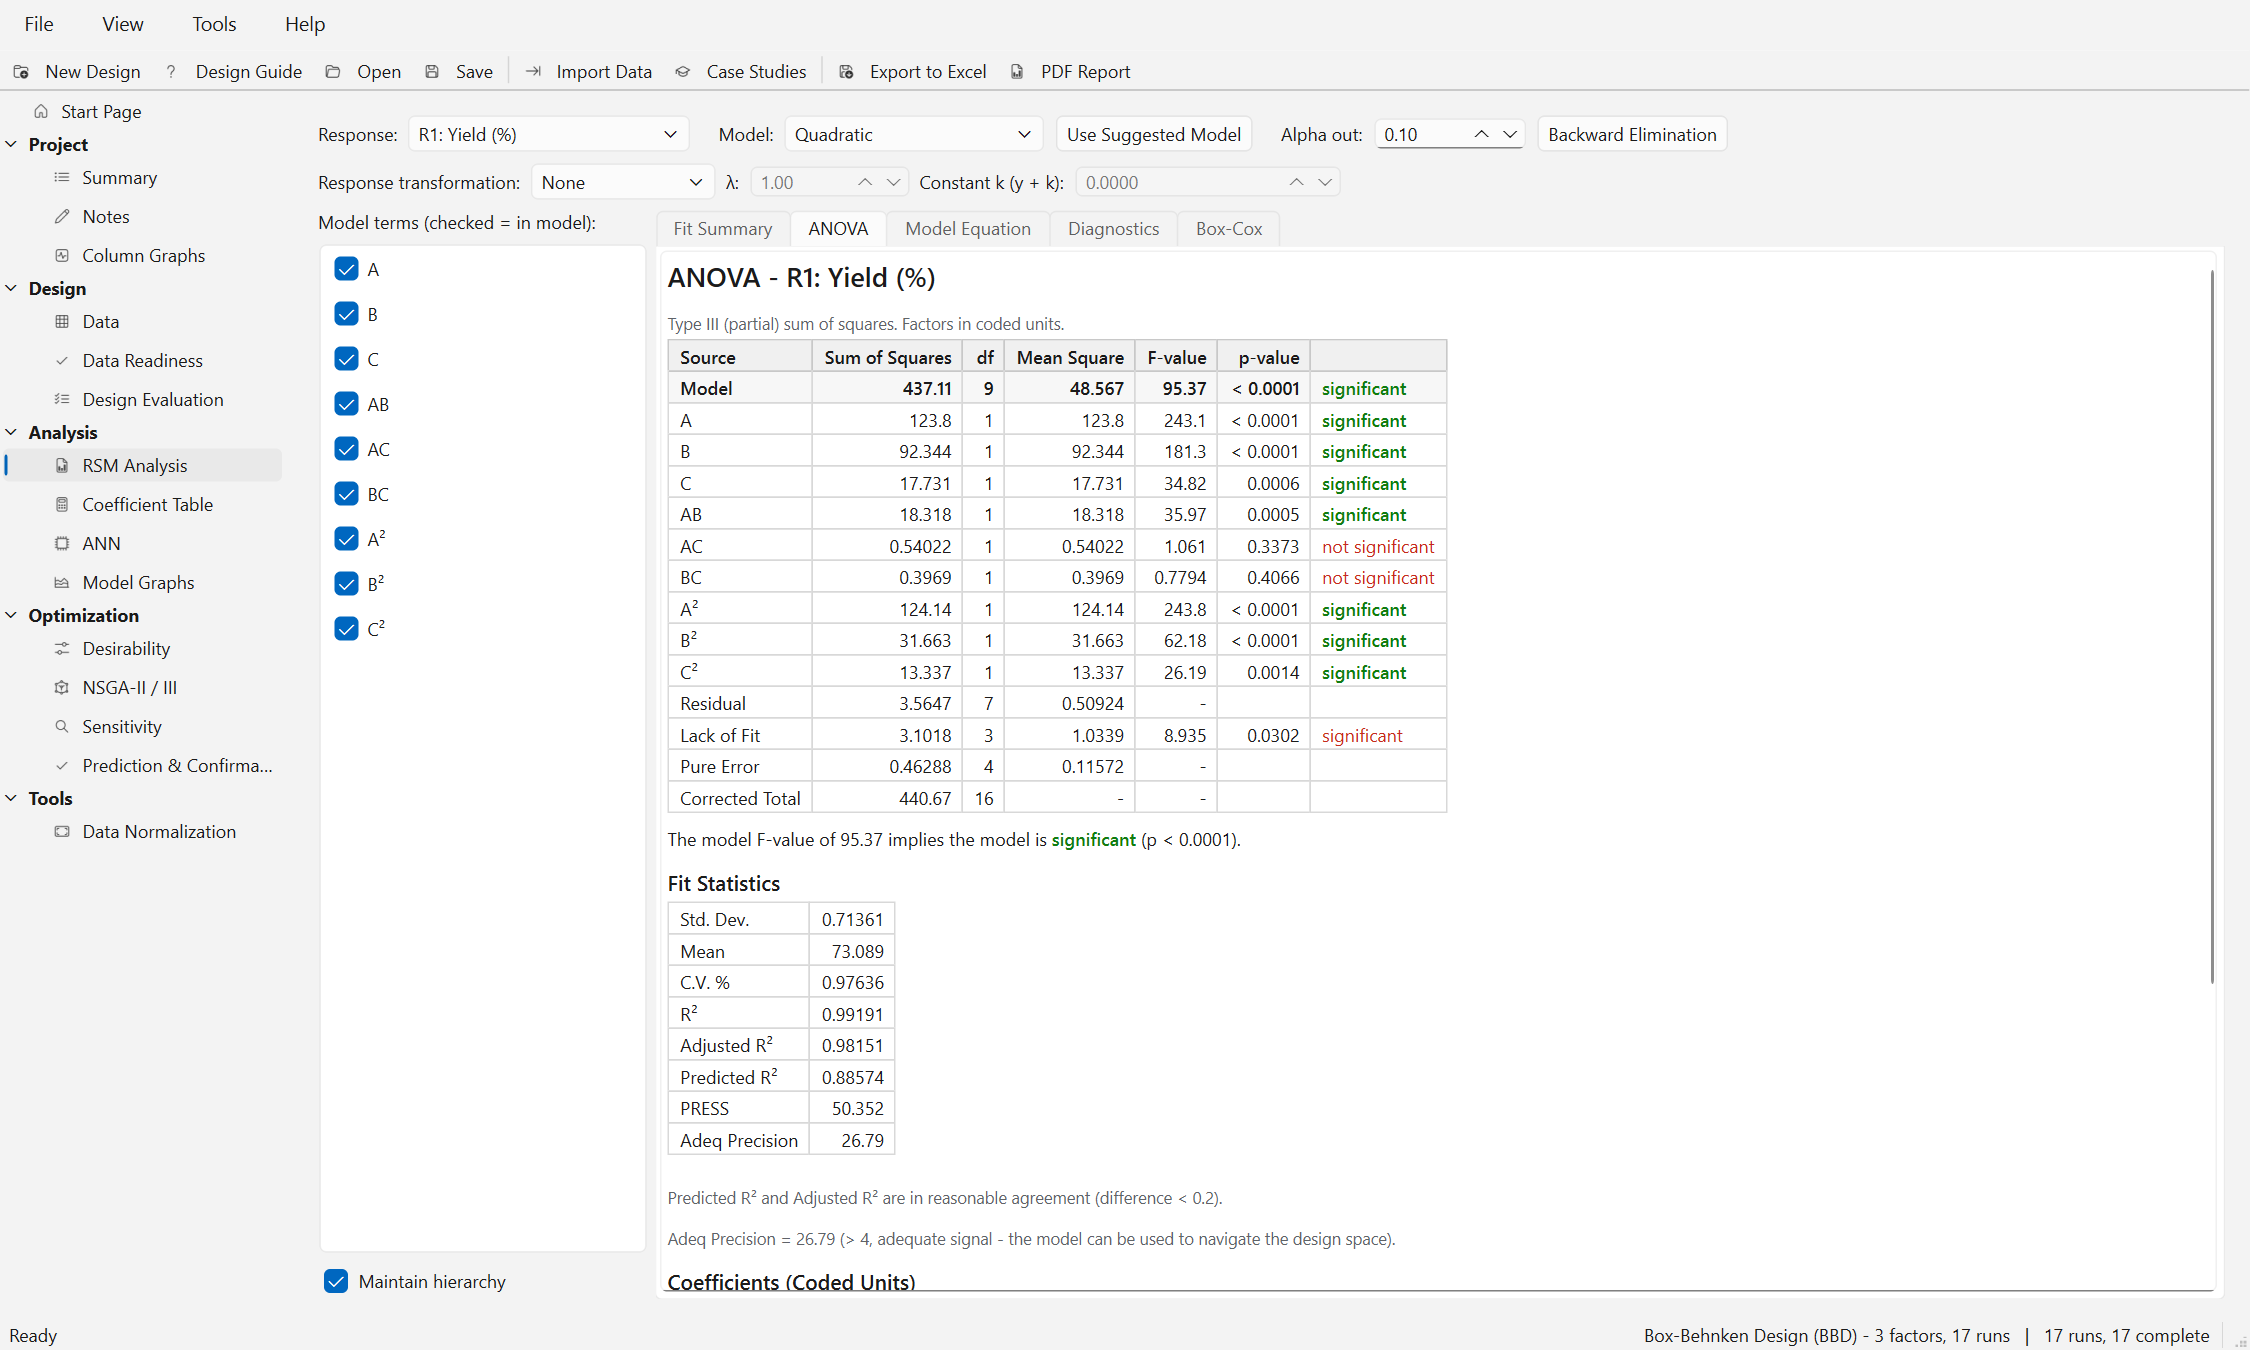
\includegraphics[width=\linewidth]{rsm_anova.png}
\caption{ANOVA sub-tab for Yield (Box-Behnken extraction case, quadratic model): Type III ANOVA with lack
of fit and pure error, model sentence, fit statistics and the notes below them.}
\label{fig:ch05-anova}
\end{figure}

\subsection*{Output and how to read it}
\begin{enumerate}
  \item Header notes: ``Type III (partial) sum of squares.'' and either ``Factors in coded units.'' or
        ``Scheffé model in pseudo-components.'', plus the transformation and the block note if present.
  \item The ANOVA table with the columns \ui{Source}, \ui{Sum of Squares}, \ui{df}, \ui{Mean Square},
        \ui{F-value}, \ui{p-value} and a verdict (``significant'' when $p<0.05$, otherwise ``not
        significant''). Green means good: $p<0.05$ for the model and the terms, $p\ge0.05$ for lack of
        fit. Rows: \ui{Block} (if any), \ui{Model}, \ui{Linear Mixture} (mixture models), one row per
        term, \ui{Residual}, \ui{Lack of Fit} and \ui{Pure Error} (when both have degrees of freedom) and
        \ui{Corrected Total}.
  \item A sentence on the model: ``The model F-value of \dots{} implies the model is significant (p
        \dots).'' or ``The model is not significant relative to noise.''
  \item \ui{Fit Statistics} (Table~\ref{tab:ch05-fitstats}) with two notes on the agreement of adjusted
        and predicted R² and on Adeq Precision.
  \item \ui{Coefficients (Coded Units)} or \ui{Coefficients (Pseudo-components)}: \ui{Term},
        \ui{Estimate}, \ui{df} (always 1 per column), \ui{Std. Error}, \ui{95\% CI Low}, \ui{95\% CI High}
        and \ui{VIF}. The p-values of the individual coefficients are on the \ui{Coefficient Table} page.
  \item Notes on mixture models, effect coding and the Shapiro-Wilk test of the residuals
        (Section~\ref{sec:ch05-diag}).
\end{enumerate}
p-values are printed with 4 decimals, or as ``$<$ 0.0001''.

\subsection*{Theory as implemented}
Let SST be the corrected total sum of squares and $\text{SSE}(S)$ the residual sum of squares of the model
with the column set $S$. The table is built as follows \citep{montgomery2017,myers2016}:
\begin{align}
  \text{SS}_{\text{Block}}&=\text{SST}-\text{SSE}(\mathbf 1,\text{blocks}), \label{eq:ch05-ssblock}\\
  \text{SS}_{\text{Model}}&=\text{SST}-\text{SS}_{\text{Block}}-\text{SSE}, \qquad
  F_{\text{Model}}=\frac{\text{SS}_{\text{Model}}/df_M}{\text{MSE}}, \label{eq:ch05-ssmodel}\\
  \text{SS}_t&=\text{SSE}(X\text{ without the columns of }t)-\text{SSE}, \qquad
  F_t=\frac{\text{SS}_t/df_t}{\text{MSE}}. \label{eq:ch05-sstype3}
\end{align}
$df_M$ is the number of term columns ($p-1$ for intercept-free mixture models) and $df_t$ the number of
columns of term $t$ (for example $L-1$ for a categoric main effect). Equation~\eqref{eq:ch05-sstype3} is
the partial (Type III) sum of squares: each term is tested after all other terms, so the term SS do not
add up to the model SS when the design is not orthogonal. The block SS in
\eqref{eq:ch05-ssblock} is sequential: blocks are removed first and the block columns stay in every reduced
model. Sequential sums of squares between model orders are used in the Fit Summary
(Equation~\ref{eq:ch05-seqF}).

\paragraph{Mixture models.} The linear blending terms are not tested one by one, because in a Scheffé model
they are not effects in the usual sense. They are tested together in the \ui{Linear Mixture} row:
\begin{equation}
  \text{SS}_{\text{lin}}=\text{SSE}(\mathbf 1+\text{non-linear terms})-\text{SSE}_{\text{full}},\qquad
  df_{\text{lin}}=q-1,
  \label{eq:ch05-linmix}
\end{equation}
with $q$ the number of linear blending columns. The note says ``In mixture models the linear terms are not
tested individually; they are tested together in the Linear Mixture row.''

\paragraph{Pure error and lack of fit.} Runs with identical coded settings (rounded to 6 decimals) in the
same block form a replicate group $g$. Then
\begin{equation}
  \text{SS}_{\text{PE}}=\sum_g\sum_{i\in g}(y_i-\bar y_g)^2,\quad df_{\text{PE}}=\sum_g(n_g-1),\qquad
  \text{SS}_{\text{LOF}}=\text{SSE}-\text{SS}_{\text{PE}},\quad df_{\text{LOF}}=(n-p)-df_{\text{PE}},
  \label{eq:ch05-lof}
\end{equation}
and $F_{\text{LOF}}=\text{MS}_{\text{LOF}}/\text{MS}_{\text{PE}}$ ($p=0$ is reported if the pure error is
exactly zero). Lack of fit is judged at $\alpha=0.05$ everywhere in the program.

\subsection*{Fit statistics}
Let $D=\text{SST}-\text{SS}_{\text{Block}}$ and $\bar y$ the mean of the (transformed) response.
Table~\ref{tab:ch05-fitstats} gives the exact formulas.

\begin{table}[htbp]\centering\small
\caption{Fit statistics on the ANOVA sub-tab ($n$ runs, $p$ columns, $df_M$ model df, $df_R=n-p$).}
\label{tab:ch05-fitstats}
\begin{tabularx}{\linewidth}{@{}l l X@{}}
\toprule
Label & Formula & Remark \\
\midrule
\ui{Std. Dev.} & $\sqrt{\text{MSE}}$ & residual standard deviation \\
\ui{Mean} & $\bar y$ & on the transformed scale \\
\ui{C.V. \%} & $100\sqrt{\text{MSE}}/|\bar y|$ & \\
\ui{R²} & $1-\text{SSE}/D$ & \\
\ui{Adjusted R²} & $1-\text{MSE}\big/\big(D/(df_M+df_R)\big)$ & penalizes the number of terms \\
\ui{Predicted R²} & $1-\text{PRESS}/D$ & not shown if a run has $h_{ii}>1-10^{-10}$ \\
\ui{PRESS} & $\sum_i\big(e_i/(1-h_{ii})\big)^2$ & leave-one-out prediction errors \citep{allen1974} \\
\ui{Adeq Precision} & $(\max_i\hat y_i-\min_i\hat y_i)\big/\sqrt{p\,\text{MSE}/n}$ & signal-to-noise ratio \\
\bottomrule
\end{tabularx}
\end{table}

PRESS uses the fact that the leave-one-out residual of run $i$ equals $e_i/(1-h_{ii})$, so no refitting is
needed \citep{allen1974}. Adeq Precision compares the range of the fitted values with the average standard
error of prediction at the design points: since $\sum_i h_{ii}=p$, the average prediction variance is
$p\,\text{MSE}/n$. The notes below the table read:
\begin{itemize}
  \item ``Predicted R² and Adjusted R² are in reasonable agreement (difference $<$ 0.2).'' or ``\dots
        differ by more than 0.2 - check for outliers or simplify the model.'' The program tests
        Adjusted R² minus Predicted R².
  \item ``Adeq Precision = \dots{} ($>$ 4, adequate signal - the model can be used to navigate the design
        space).'' or ``($\le$ 4, weak signal).''
\end{itemize}

The 95\% confidence interval of a coefficient is $\hat\beta_j\pm t_{0.975,\,n-p}\,\text{se}(\hat\beta_j)$.

\subsection*{What to do when a check fails}
\begin{itemize}
  \item \emph{Model not significant}: the factors explain no more than noise. Check the data entry,
        consider a lower order or accept that the factors have no effect in this range.
  \item \emph{Significant lack of fit}: try the next order, a transformation, or an ANN model; but first
        look at the size of the pure error (see the example).
  \item \emph{Adjusted and predicted R² differ by more than 0.2}: look for influential runs on the
        Diagnostics sub-tab and remove unnecessary terms.
\end{itemize}

\subsection*{Example: Box-Behnken extraction, Yield (quadratic)}
Figure~\ref{fig:ch05-anova} shows the result. The model has $F=95.37$ ($p<0.0001$). All main effects, AB
($F=35.97$, $p=0.0005$) and the three squares are significant; AC ($p=0.3373$) and BC ($p=0.4066$) are not.
The residual SS is 3.5647 on 7 df. Lack of fit is significant: $F=8.935$ on 3 and 4 df, $p=0.0302$. This
does not mean that the model is poor: the pure error comes from the 5 center points only and is very small
($\text{MS}_{\text{PE}}=0.1157$, a standard deviation of 0.34), while the residual standard deviation is
0.714. With so little pure-error information the lack-of-fit test reacts to small systematic deviations.
The other statistics are Std.\ Dev.\ 0.71361, Mean 73.089, C.V.\ 0.976\%, R² 0.99191, Adjusted R² 0.98151,
Predicted R² 0.88574 (PRESS 50.35) and Adeq Precision 26.79. Adjusted and predicted R² differ by 0.096, so
they agree. The coefficient table gives, for example, $A=3.9337$ with standard error 0.2523.

\subsection*{Example: mixture}
For \emph{Edible Film Formulation (Mixture)}, Tensile Strength, quadratic Scheffé model: Model $F=415.76$,
Linear Mixture SS 74.75 on 2 df ($F=561.0$), AB $F=96.56$, AC $F=212.5$, BC $F=6.19$ ($p=0.0377$), lack of
fit $p=0.0993$ (not significant), R² 0.99617, Adjusted R² 0.99377, Predicted R² 0.99122.

\begin{figure}[htbp]\centering
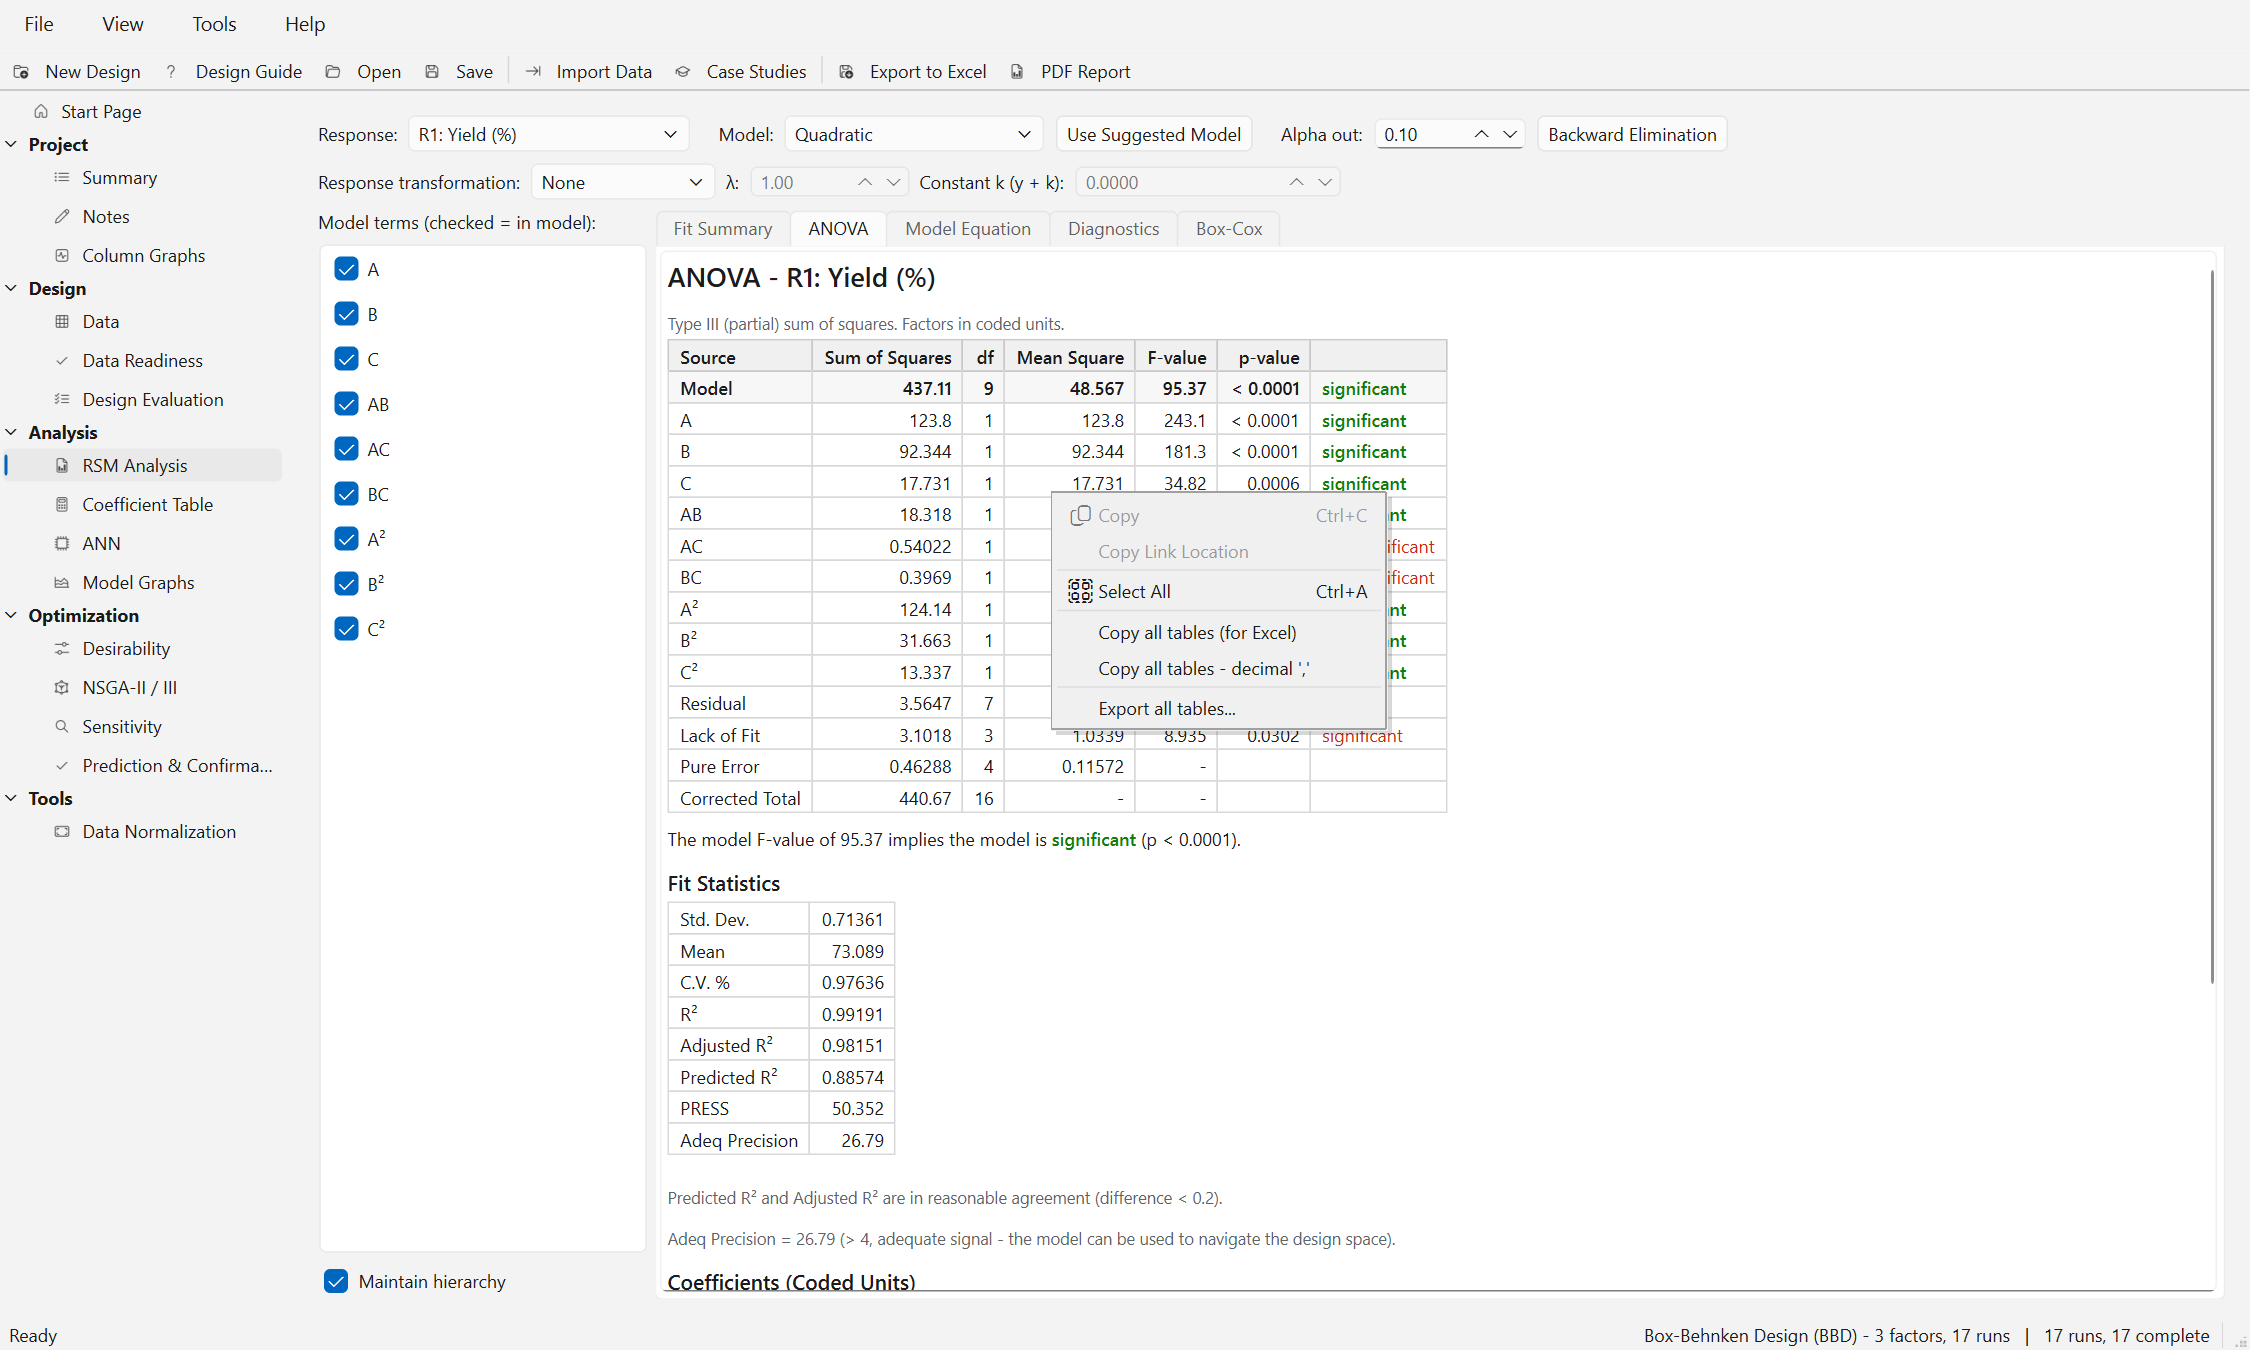
\includegraphics[width=0.75\linewidth]{report_context_menu.png}
\caption{Right-click menu of a report sub-tab: copy all tables to Excel (with either decimal separator) or
export them to a file.}
\label{fig:ch05-reportmenu}
\end{figure}

\subsection*{Data export}
Right-click any report sub-tab (Fit Summary, ANOVA, Model Equation, GLM or REML) for
\ui{Copy all tables (for Excel)}, \ui{Copy all tables - decimal ','} and \ui{Export all tables\dots}
(Figure~\ref{fig:ch05-reportmenu}). The export writes one Excel sheet per table, or a CSV file.

\section{Model equation}\label{sec:ch05-equation}

\subsection*{Purpose}
The \ui{Model Equation} sub-tab writes the fitted model as an equation that can be used outside the
program.

\begin{figure}[htbp]\centering
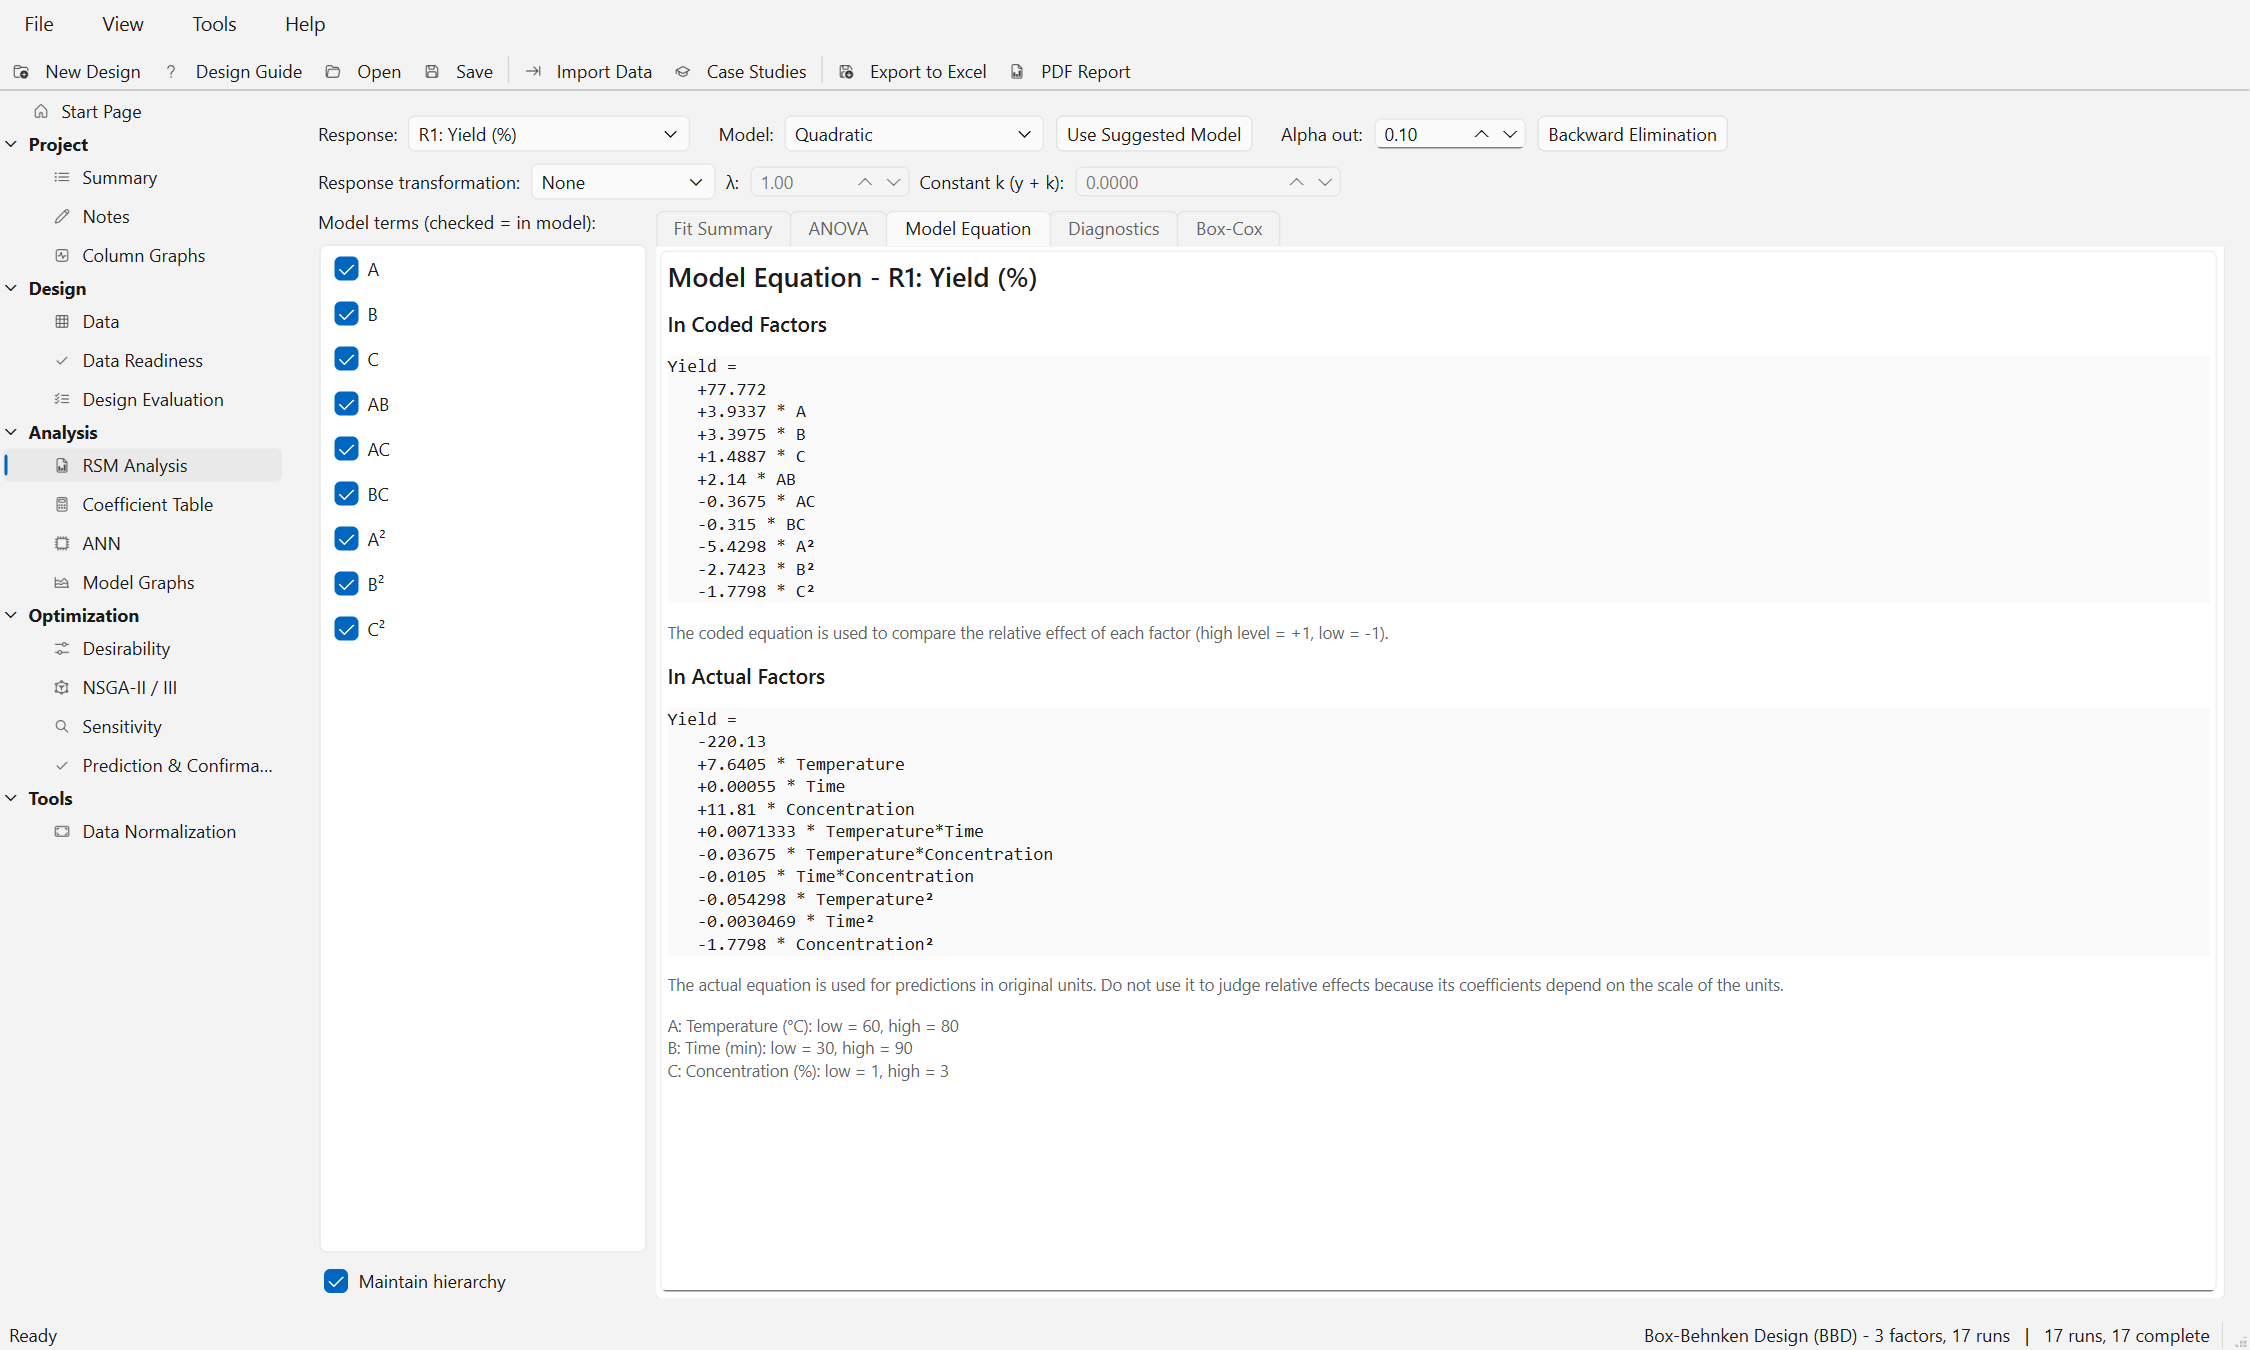
\includegraphics[width=\linewidth]{rsm_equation.png}
\caption{Model Equation sub-tab for Yield: the equation in coded factors and in actual factors.}
\label{fig:ch05-equation}
\end{figure}

\subsection*{Output and how to read it}
\begin{itemize}
  \item \ui{In Coded Factors}: the coefficients for factors coded $-1$ to $+1$. Note: ``The coded
        equation is used to compare the relative effect of each factor (high level = +1, low = -1).''
  \item \ui{In Actual Factors}: the same model in the original units, one block per combination of
        categoric levels (for example \ui{In Actual Factors - Solvent = Methanol}). Note: ``The actual
        equation is used for predictions in original units. Do not use it to judge relative effects
        because its coefficients depend on the scale of the units.''
  \item Mixture designs show \ui{In Pseudo-components}, with the note ``Pseudo-component: x = (amount
        $-$ lower limit) / (total $-$ $\Sigma$ lower limits). Linear coefficients = predicted response
        of the pure blends (vertices).'' \ui{In Actual Components} is shown only when every lower limit is
        0 and the design is not combined; otherwise a note says to use the pseudo-component equation. For
        combined mixture-process designs the note gives the reason: ``The equation in actual units is not
        given for combined mixture-process designs: the model crosses the mixture terms with the process
        terms, and the conversion to actual units is only done for mixture models without process factors.
        Use the equation above (pseudo-components, process factors coded $-1$ to $+1$).''
  \item The left-hand side shows the transformation, for example \ui{Ln(Yield)}, \ui{Sqrt(Yield)},
        \ui{(Yield +5)} for a constant $k=5$, \ui{logit(p Germinated)} for logistic and
        \ui{ln($\lambda$ \dots)} for Poisson regression.
  \item A legend lists the factor ranges (and the mixture total). With blocks: ``The equation applies to
        the average of all blocks.''
\end{itemize}

\subsection*{Theory as implemented}
Substituting \eqref{eq:ch05-coding} as $z_j=a_jx_j+b_j$ with $a_j=1/h_j$ and $b_j=-c_j/h_j$ into each
monomial and expanding binomially,
\begin{equation}
  \prod_j z_j^{e_j}=\prod_j\sum_{m=0}^{e_j}\binom{e_j}{m}a_j^{m}b_j^{\,e_j-m}x_j^{m},
  \label{eq:ch05-coded2actual}
\end{equation}
gives the actual coefficients. Categoric columns are first replaced by their values at the chosen level
(+1, $-1$ or 0, Equation~\ref{eq:ch05-effectcode}). For mixtures with all lower limits 0 the actual
coefficient of a term of degree $d$ is $\beta/T^{d}$.

\subsection*{Example}
For Yield of the Box-Behnken case (Figure~\ref{fig:ch05-equation}):
\begin{multline*}
\text{Yield}=77.772+3.9337A+3.3975B+1.4887C+2.14AB-0.3675AC\\
-0.315BC-5.4298A^2-2.7423B^2-1.7798C^2
\end{multline*}
in coded units, and in actual units (Temperature $T$, Time $t$, Concentration $c$)
\begin{multline*}
\text{Yield}=-220.13+7.6405\,T+0.00055\,t+11.81\,c+0.0071333\,Tt-0.03675\,Tc\\
-0.0105\,tc-0.054298\,T^2-0.0030469\,t^2-1.7798\,c^2.
\end{multline*} The coefficient of Time in actual units is
almost zero although Time is the second most important factor: actual coefficients cannot be compared.
For the categoric case the three actual equations differ only in the intercept and in the coefficients
of Temperature and Time, for example intercept $-48.211$ (Ethanol), $-51.117$ (Methanol) and $-51.911$
(Acetone).

\section{Backward elimination}\label{sec:ch05-backward}

\subsection*{Purpose}
Backward elimination removes terms that do not contribute significantly, to obtain a smaller model with
better prediction properties.

\subsection*{How to use}
\begin{enumerate}
  \item Choose the starting model (order and terms).
  \item Set \ui{Alpha out:} (default 0.10).
  \item Click \ui{Backward Elimination}. The term list shows the result; undo by selecting the order again
        in \ui{Model:} (this restores all terms).
\end{enumerate}

\subsection*{Rule as implemented}
\begin{enumerate}
  \item Fit the current terms. If the residual df is 0, stop (a saturated model is not reduced).
  \item Candidates are the terms with a p-value larger than $\alpha_{\text{out}}$: the Type III F test for
        least squares, the likelihood-ratio test for GLM, the Wald F test for REML.
  \item A term is not a candidate if it is a linear mixture term or, when \ui{Maintain hierarchy} is checked
        (the default), if it is contained in another term that is still in the model. With the check box
        cleared, any term with $p>\alpha_{\text{out}}$ can be removed, and the result may be a
        non-hierarchical model.
  \item Remove the candidate with the largest p-value, refit and repeat until no candidate is left.
\end{enumerate}
Because the p-values change after each removal, removing terms one at a time is safer than removing all
non-significant terms at once.

\subsection*{Examples}
\begin{itemize}
  \item Box-Behnken, Yield, quadratic, $\alpha_{\text{out}}=0.10$: BC and then AC are removed; the model
        A, B, C, AB, A², B², C² remains. For Purity the same procedure removes B² first ($p=0.9745$
        in the full model) and then AC and BC.
  \item Germination (logistic): only B² is removed (likelihood-ratio $p=0.5312$); AB stays because its
        $p=0.0622$ is below 0.10.
  \item Oven hardness (split-plot): AC and BC are removed; A, B, C, AB remain.
\end{itemize}

\section{Response transformations and Box-Cox}\label{sec:ch05-transform}

\subsection*{Purpose}
A transformation can make the residual variance constant, the residuals more normal and the model simpler.
The Box-Cox plot shows which power transformation the data support.

\subsection*{Transformations}
The constant $k$ (\ui{Constant k (y + k):}) is added first, $v=y+k$. Then:

\begin{center}\small
\begin{tabular}{@{}llll@{}}
\toprule
Option & Forward & Requirement & Equation label \\
\midrule
None & $y$ & -- & \ui{Yield} \\
Square root & $\sqrt v$ & all $v\ge0$ & \ui{Sqrt(Yield)} \\
Natural log (ln) & $\ln v$ & all $v>0$ & \ui{Ln(Yield)} \\
Base 10 log & $\log_{10}v$ & all $v>0$ & \ui{Log10(Yield)} \\
Inverse (1/y) & $1/v$ & all $v>0$ & \ui{1/(Yield)} \\
Power (y\^{}$\lambda$) & $v^\lambda$ ($\ln v$ if $\lambda=0$) & all $v>0$ & \ui{(Yield)\^{}$\lambda$} \\
\bottomrule
\end{tabular}
\end{center}

All statistics (ANOVA, R², Std.\ Dev., Mean) refer to the transformed scale. Predictions, confidence and
prediction intervals are computed on the transformed scale, back-transformed (the inverse power uses
$\text{sign}(z)|z|^{1/\lambda}$), $k$ is subtracted, and the interval limits are sorted (the inverse
transformation reverses their order). Graphs and optimization therefore work in the original units.
The transformation box is disabled for binomial and Poisson responses.

\subsection*{How to use the Box-Cox sub-tab}
\begin{enumerate}
  \item Select the model first; the Box-Cox plot is computed for the current terms (and blocks).
  \item If any response value is $\le0$, choose a transformation and enter a constant $k$ that makes all
        $y+k>0$; the plot then refers to $y+k$ (the x-axis label shows ``transform of y +k'').
  \item Read the recommendation below the plot and click \ui{Apply Recommendation} to set the
        transformation (and $\lambda$ for Power). The constant $k$ is not changed.
\end{enumerate}

\begin{figure}[htbp]\centering
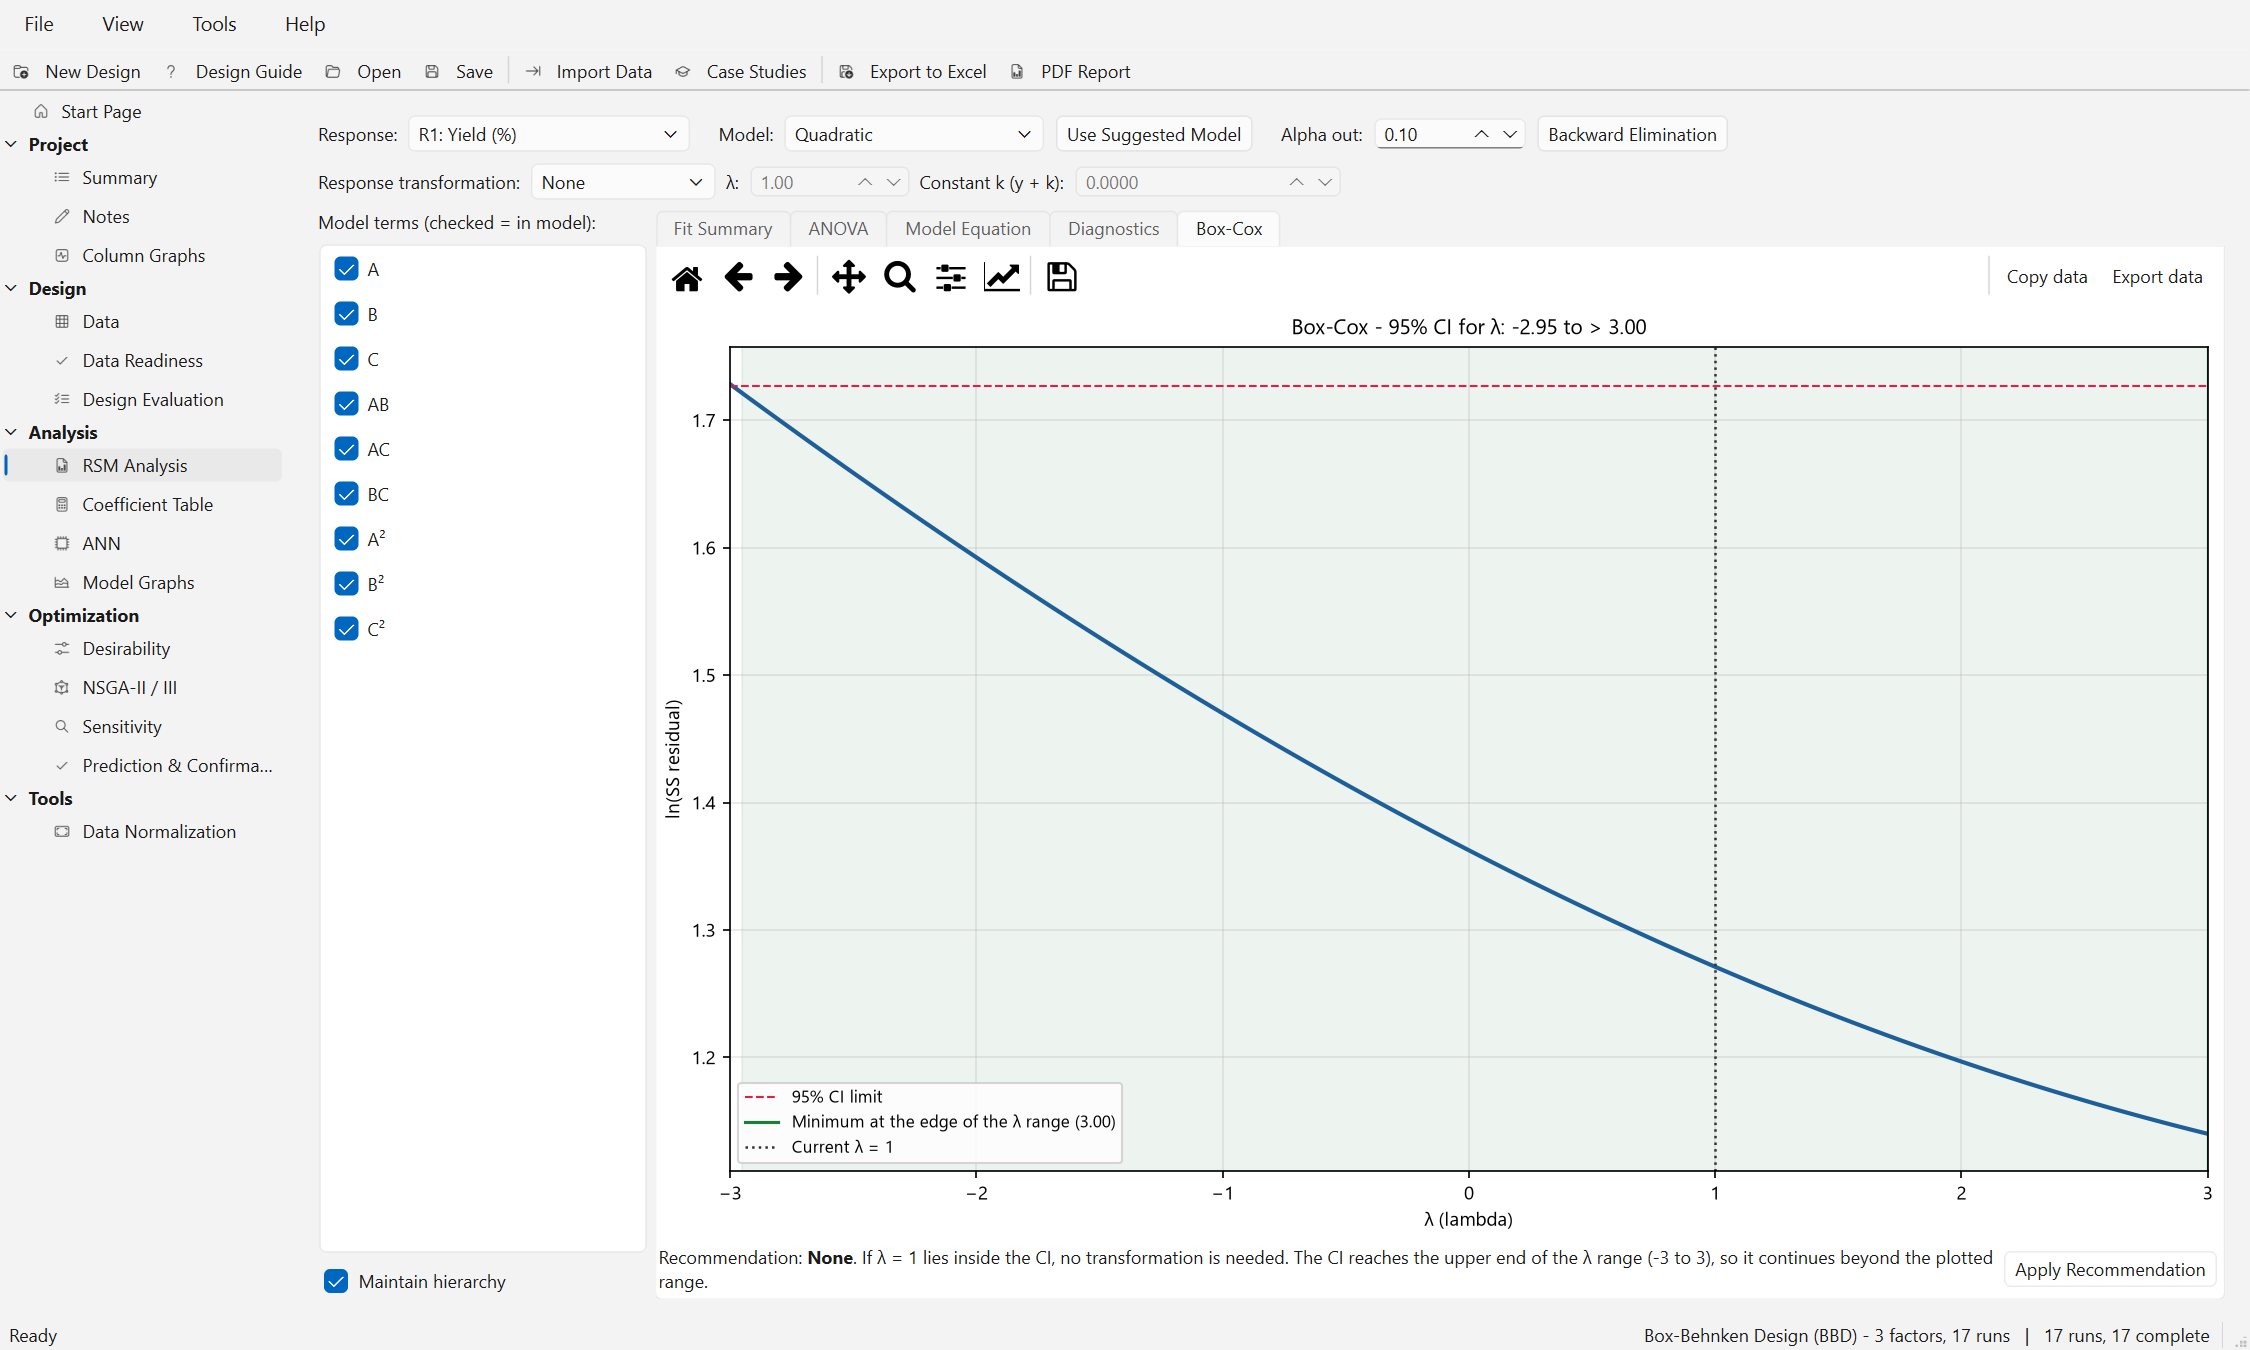
\includegraphics[width=\linewidth]{rsm_boxcox.png}
\caption{Box-Cox sub-tab for Yield (Box-Behnken case): ln(SS residual) against $\lambda$ with the 95\%
limit, the confidence band and the recommendation ``None''.}
\label{fig:ch05-boxcox}
\end{figure}

\subsection*{Theory as implemented}
For each $\lambda$ on the grid $-3,-2.95,\dots,3$ (121 values) the scaled power transformation
\begin{equation}
  w^{(\lambda)}=\begin{cases}\dfrac{v^\lambda-1}{\lambda\,\dot v^{\lambda-1}}, & \lambda\neq0,\\[1ex]
  \dot v\ln v, & \lambda=0,\end{cases}\qquad \dot v=\exp\Big(\frac1n\sum\ln v_i\Big),
  \label{eq:ch05-boxcox}
\end{equation}
is regressed on the current model matrix, and the residual sum of squares $\text{SS}(\lambda)$ is computed
\citep{boxcox1964}. The geometric mean $\dot v$ makes the SS comparable across $\lambda$, so maximizing the
likelihood is the same as minimizing $\text{SS}(\lambda)$: the profile log-likelihood is
$\ell(\lambda)=-\tfrac n2\ln\text{SS}(\lambda)+\text{const}$. The plot shows $\ln\text{SS}(\lambda)$; the
best $\lambda$ is the grid minimum. The approximate 95\% confidence interval contains all $\lambda$ with
\begin{equation}
  \ln\text{SS}(\lambda)\le\ln\text{SS}(\hat\lambda)+\ln\!\Big(1+\frac{t^2_{0.975,\nu}}{\nu}\Big),
  \qquad \nu=n-p,
  \label{eq:ch05-boxcoxci}
\end{equation}
which is the usual $\text{SS}^{*}=\text{SS}(\hat\lambda)(1+t^2_{\alpha/2,\nu}/\nu)$ rule
\citep{montgomery2017,boxcox1964}.

\paragraph{Recommendation rule.}
\begin{enumerate}
  \item If $\lambda=1$ lies in the CI: \emph{None}.
  \item Otherwise the first of $\lambda=0.5$ (\emph{Square root}), $0$ (\emph{Natural log}) and $-1$
        (\emph{Inverse}) that lies in the CI.
  \item Otherwise \emph{Power} with the best $\lambda$ rounded to 2 decimals, unless the minimum lies at the
        edge of the grid; then no recommendation is given.
\end{enumerate}

\paragraph{Plot and messages.} The blue curve is $\ln\text{SS}$; the dashed red line labeled ``95\% CI
limit'' is the threshold of \eqref{eq:ch05-boxcoxci} and the green band the CI. A green vertical line marks
``Best $\lambda$ = \dots'' or, when the minimum is at the end of the grid, ``Minimum at the edge of the
$\lambda$ range (\dots)''. A dotted line marks the current $\lambda$ (1 for none, 0.5, 0 for both logs, $-1$,
or the power). The title reads ``Box-Cox - 95\% CI for $\lambda$: lo to hi''; a limit that reaches the end of
the grid is written ``$<$ -3.00'' or ``$>$ 3.00''. The text below the plot gives the recommendation and adds
``The CI reaches the upper end of the $\lambda$ range (-3 to 3), so it continues beyond the plotted range.''
when this happens. If the minimum is at the edge and no standard value is in the CI, the text explains that
no reliable $\lambda$ can be given and advises to check the model (lack of fit, outliers) first. Box-Cox is
not available for binomial, Poisson or split-plot responses (``Box-Cox is not available for this
response.''), and needs at least 3 values with all $y+k>0$.

\subsection*{Examples}
\begin{itemize}
  \item Box-Behnken, Yield (Figure~\ref{fig:ch05-boxcox}): the curve is very flat, the CI is $-2.95$ to
        $>3.00$ and the minimum is at the upper edge ($\lambda=3$). Because $\lambda=1$ is inside the CI,
        the recommendation is \emph{None}. The response varies only between 64 and 78\%, so the data carry
        almost no information about $\lambda$.
  \item Edible film, Tensile Strength: best $\lambda=1.10$, CI 0.15 to 2.00, recommendation \emph{None}.
  \item Fermentation screening, Biomass (2FI): best $\lambda=0.90$, CI 0.45 to 1.35, recommendation
        \emph{None}.
\end{itemize}

\section{Residual diagnostics}\label{sec:ch05-diag}

\subsection*{Purpose}
The \ui{Diagnostics} sub-tab checks the assumptions of the analysis (normal, independent residuals with
constant variance) and finds runs that are outliers or have a large influence on the model.

\begin{figure}[htbp]\centering
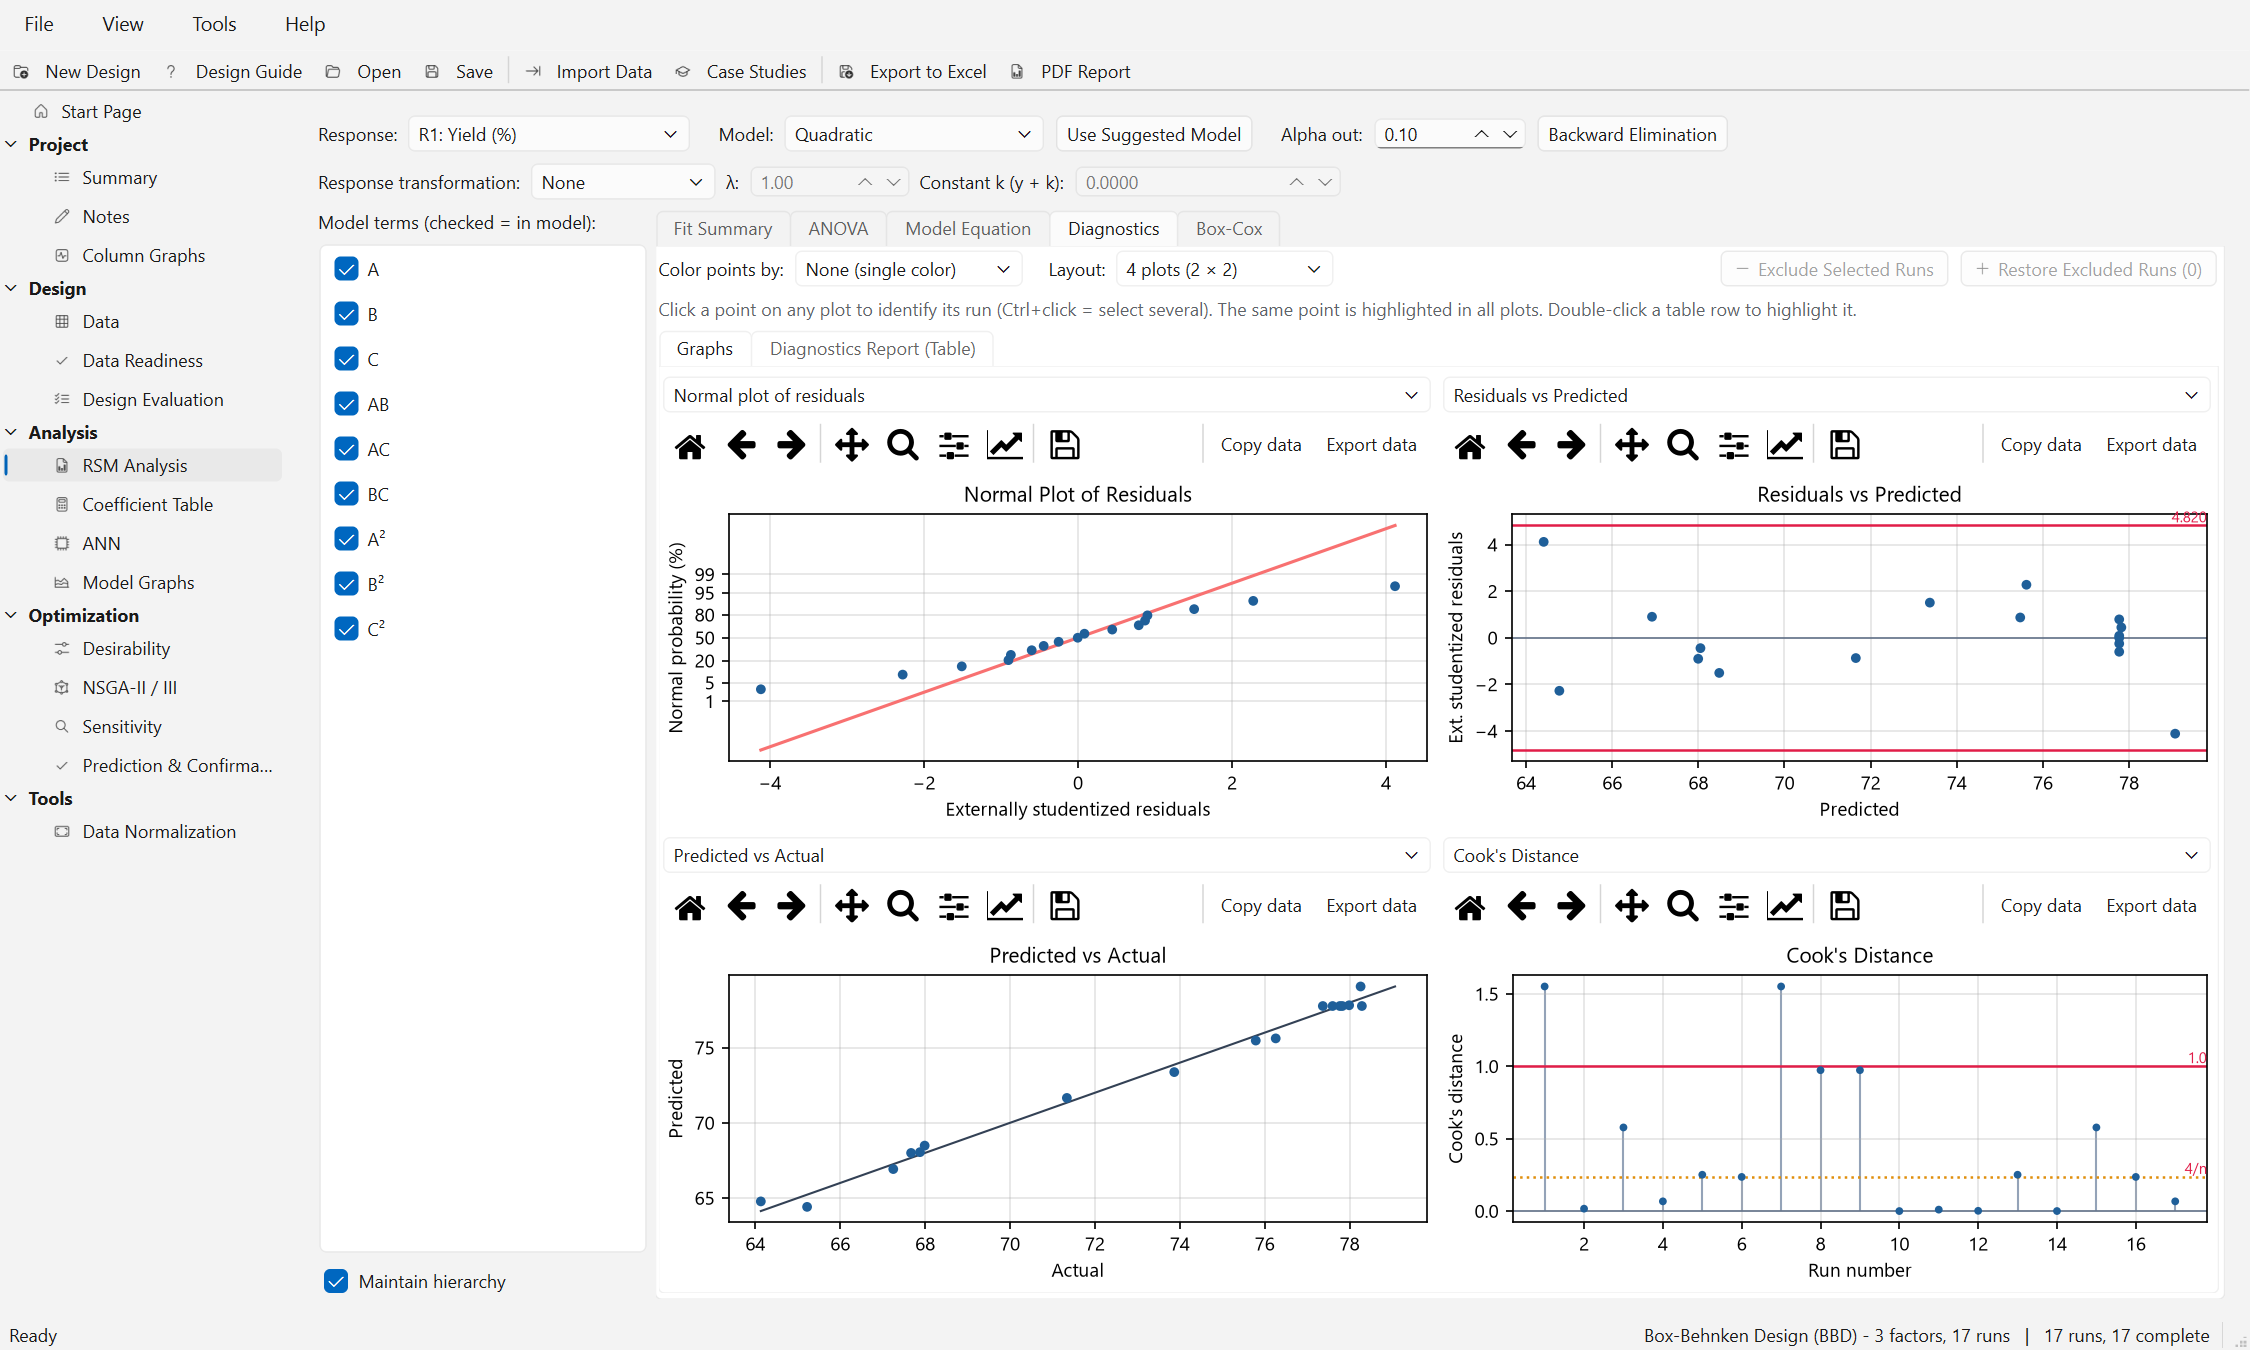
\includegraphics[width=\linewidth]{rsm_diagnostics.png}
\caption{Diagnostics sub-tab (Box-Behnken case, Yield) with the default four plots: normal plot, residuals
versus predicted with the Bonferroni limits, predicted versus actual and Cook's distance.}
\label{fig:ch05-diag}
\end{figure}

\subsection*{How to use}
\begin{enumerate}
  \item Choose the plots: each of the four panels has its own selector (Table~\ref{tab:ch05-diagplots}) and
        its own plot toolbar.
  \item Optionally color the points with \ui{Color points by:} and change the number of panels with
        \ui{Layout:}.
  \item Click a point to identify its run; the same run is circled and labeled in every plot, and the text
        above the plots shows its actual and predicted value, externally studentized residual, leverage and
        Cook's distance. Ctrl+click (or Shift+click) selects several runs. Clicking away from the points
        clears the selection. Clicks are ignored while the zoom or pan tool of the plot toolbar is active.
  \item Open the inner tab \ui{Diagnostics Report (Table)} for all numbers. Double-click a row to highlight
        that run in the plots.
  \item To leave runs out of the analysis, select them and click \ui{Exclude Selected Runs}; restore them
        with \ui{Restore Excluded Runs (N)}.
\end{enumerate}

\begin{table}[htbp]\centering\small
\caption{Options of the Diagnostics sub-tab.}\label{tab:ch05-diagopts}
\begin{tabularx}{\linewidth}{@{}>{\raggedright\arraybackslash}p{2.4cm} >{\raggedright\arraybackslash}p{3.8cm} >{\raggedright\arraybackslash}p{3.0cm} X@{}}
\toprule
Option & Values & Default & Meaning \\
\midrule
\ui{Color points by:} & None (single color), each factor, Run order, Predicted value & None & Numeric values use a continuous color scale with a color bar; categoric factors one color per level with a legend. \\
\ui{Layout:} & 4 plots (2 $\times$ 2), 2 plots side by side, 1 large plot & 4 plots & Number of panels shown. \\
Panel selector & see Table~\ref{tab:ch05-diagplots} & Normal plot, Residuals vs Predicted, Predicted vs Actual, Cook's Distance & Plot in each panel. \\
\bottomrule
\end{tabularx}
\end{table}

\begin{table}[htbp]\centering\small
\caption{Diagnostic plots available in each panel.}\label{tab:ch05-diagplots}
\begin{tabularx}{\linewidth}{@{}>{\raggedright\arraybackslash}p{3.4cm} X@{}}
\toprule
Plot & Content \\
\midrule
Normal plot of residuals & Sorted externally studentized residuals against $\Phi^{-1}((i-0.5)/n)$, axis in \% (1 to 99, or 0.1 to 99.9 for $n\ge200$), with the line $y=x$. Needs 3 valid points. \\
Residuals vs Predicted & Externally studentized residuals against $\hat y$ (GLM: against the linear predictor, axis ``Linear predictor (logit scale)'' or ``(log scale)''), with the zero line and the $\pm$Bonferroni limits labeled with their value. With a response transformation $\hat y$ is on the transformed scale and the axis reads ``Predicted (transformed scale)''. \\
Residuals vs Run Order & The same residuals against the run number, joined by a line (up to 400 runs). \\
Residuals vs \emph{factor} & One plot per factor; categoric levels are jittered by $\pm0.12$. \\
Predicted vs Actual & Fitted against observed values with the 45° line (transformed scale if a transformation is used; GLM: observed proportion or count against fitted probability or mean). \\
Cook's Distance & Stems against run number with a line at 1.0 and a dotted line at $4/n$ (not for REML). \\
Leverage & Stems with a line at $2p/n$. \\
DFFITS & Stems with lines at $\pm2\sqrt{p/n}$ (not for REML). \\
Histogram of residuals & Density histogram of the externally studentized residuals ($\min(40,\max(8,\lfloor n/5\rfloor))$ bins) with the standard normal density. \\
DFBETAS - \emph{term} & One plot per coefficient, lines at $\pm2/\sqrt n$ (least squares only). \\
\bottomrule
\end{tabularx}
\end{table}

\subsection*{Theory as implemented}
With $\nu=n-p$ residual degrees of freedom \citep{montgomery2017,myers2016}:
\begin{align}
  r_i&=\frac{e_i}{\sqrt{\text{MSE}(1-h_{ii})}} &&\text{(internally studentized)}, \label{eq:ch05-rint}\\
  t_i&=r_i\sqrt{\frac{\nu-1}{\nu-r_i^2}} &&\text{(externally studentized, needs } \nu>1), \label{eq:ch05-rext}\\
  D_i&=\frac{r_i^2}{p}\,\frac{h_{ii}}{1-h_{ii}} &&\text{(Cook's distance \citep{cook1977})}, \label{eq:ch05-cook}\\
  \text{DFFITS}_i&=t_i\sqrt{\frac{h_{ii}}{1-h_{ii}}}, && \label{eq:ch05-dffits}\\
  \text{DFBETAS}_{ij}&=\frac{\big[(X'X)^{-1}x_i\big]_j\,e_i/(1-h_{ii})}{s_{(i)}\sqrt{[(X'X)^{-1}]_{jj}}}
  && \text{\citep{belsley1980}}, \label{eq:ch05-dfbetas}
\end{align}
with $s_{(i)}^2=\big(\text{SSE}-e_i^2/(1-h_{ii})\big)/(\nu-1)$, the residual variance without run $i$.
The externally studentized residual is the residual of run $i$ divided by an error estimate that does not
use run $i$; under the model it follows a $t$ distribution with $\nu-1$ df. Runs with
$h_{ii}>1-10^{-10}$ (fitted exactly) get no studentized residual. DFBETAS measures how many standard errors
coefficient $j$ moves when run $i$ is deleted and is computed only for least-squares fits with $\nu>1$.

Limits used for the red cells and the plot lines:
\begin{center}\small
\begin{tabular}{@{}ll@{}}
\toprule
Statistic & Flagged when \\
\midrule
Ext.\ studentized residual & $|t_i|>t_{1-0.05/(2n),\,\nu-1}$ (Bonferroni outlier limit) \\
Leverage & $h_{ii}>2p/n$ \\
Cook's distance & $D_i>1$ (the plot also shows $4/n$) \\
DFFITS & $|\text{DFFITS}_i|>2\sqrt{p/n}$ \\
DFBETAS & $|\text{DFBETAS}_{ij}|>2/\sqrt n$ \\
\bottomrule
\end{tabular}
\end{center}

\paragraph{Normality: Shapiro-Wilk.} The ANOVA sub-tab reports the Shapiro-Wilk test of the raw residuals
\citep{shapiro1965} for $3\le n\le5000$: ``Shapiro-Wilk normality test of residuals: p = \dots{} (residuals
can be considered normal).'' when $p\ge0.05$, otherwise ``(residuals are not normal - consider a
transformation).'' With few runs the test has little power; the normal plot is more informative.

\paragraph{Independence: run order and Durbin-Watson.} Look at \ui{Residuals vs Run Order}: a trend or long
runs of residuals with the same sign suggest drift during the experiment. The Durbin-Watson statistic
$d=\sum_{i\ge2}(e_i-e_{i-1})^2/\sum_i e_i^2$ (residuals in run order, \citealp{durbin1950}) is not shown on
this page; it is computed on the \ui{Data Readiness} page, which warns when $d<1.4$, $d>2.6$ or the Spearman
trend of the residuals over the run order has $p<0.01$. Values near 2 mean no serial correlation.

\subsection*{Diagnostics report table}
The table (Figure~\ref{fig:ch05-diagtable}) has one row per analyzed run, sorted by run order, with the
columns \ui{Run}, \ui{Std}, \ui{Type}, \ui{Actual}, \ui{Predicted}, \ui{Residual}, \ui{Leverage},
\ui{Int. stud. resid.}, \ui{Ext. stud. resid.}, \ui{Cook's}, \ui{DFFITS} and one \ui{DFBETAS} column per
coefficient (least squares only). \ui{Actual} is in original units. With a response transformation the
predicted values and residuals are on the transformed scale, and the columns are then labeled
\ui{Predicted (transformed scale)} and \ui{Residual (transformed scale)}. For GLM responses the columns are \ui{Observed proportion} (or count),
\ui{Fitted probability} (or \ui{Fitted mean count}) and \ui{Deviance resid.}. Cells beyond the limits
are shaded red. The line above the table states the number of runs analyzed and excluded, each limit and
how many runs exceed it. Right-click the table to copy it (\ui{Copy entire table (for Excel)}, with either
decimal separator) or \ui{Export table\dots}.

\begin{figure}[htbp]\centering
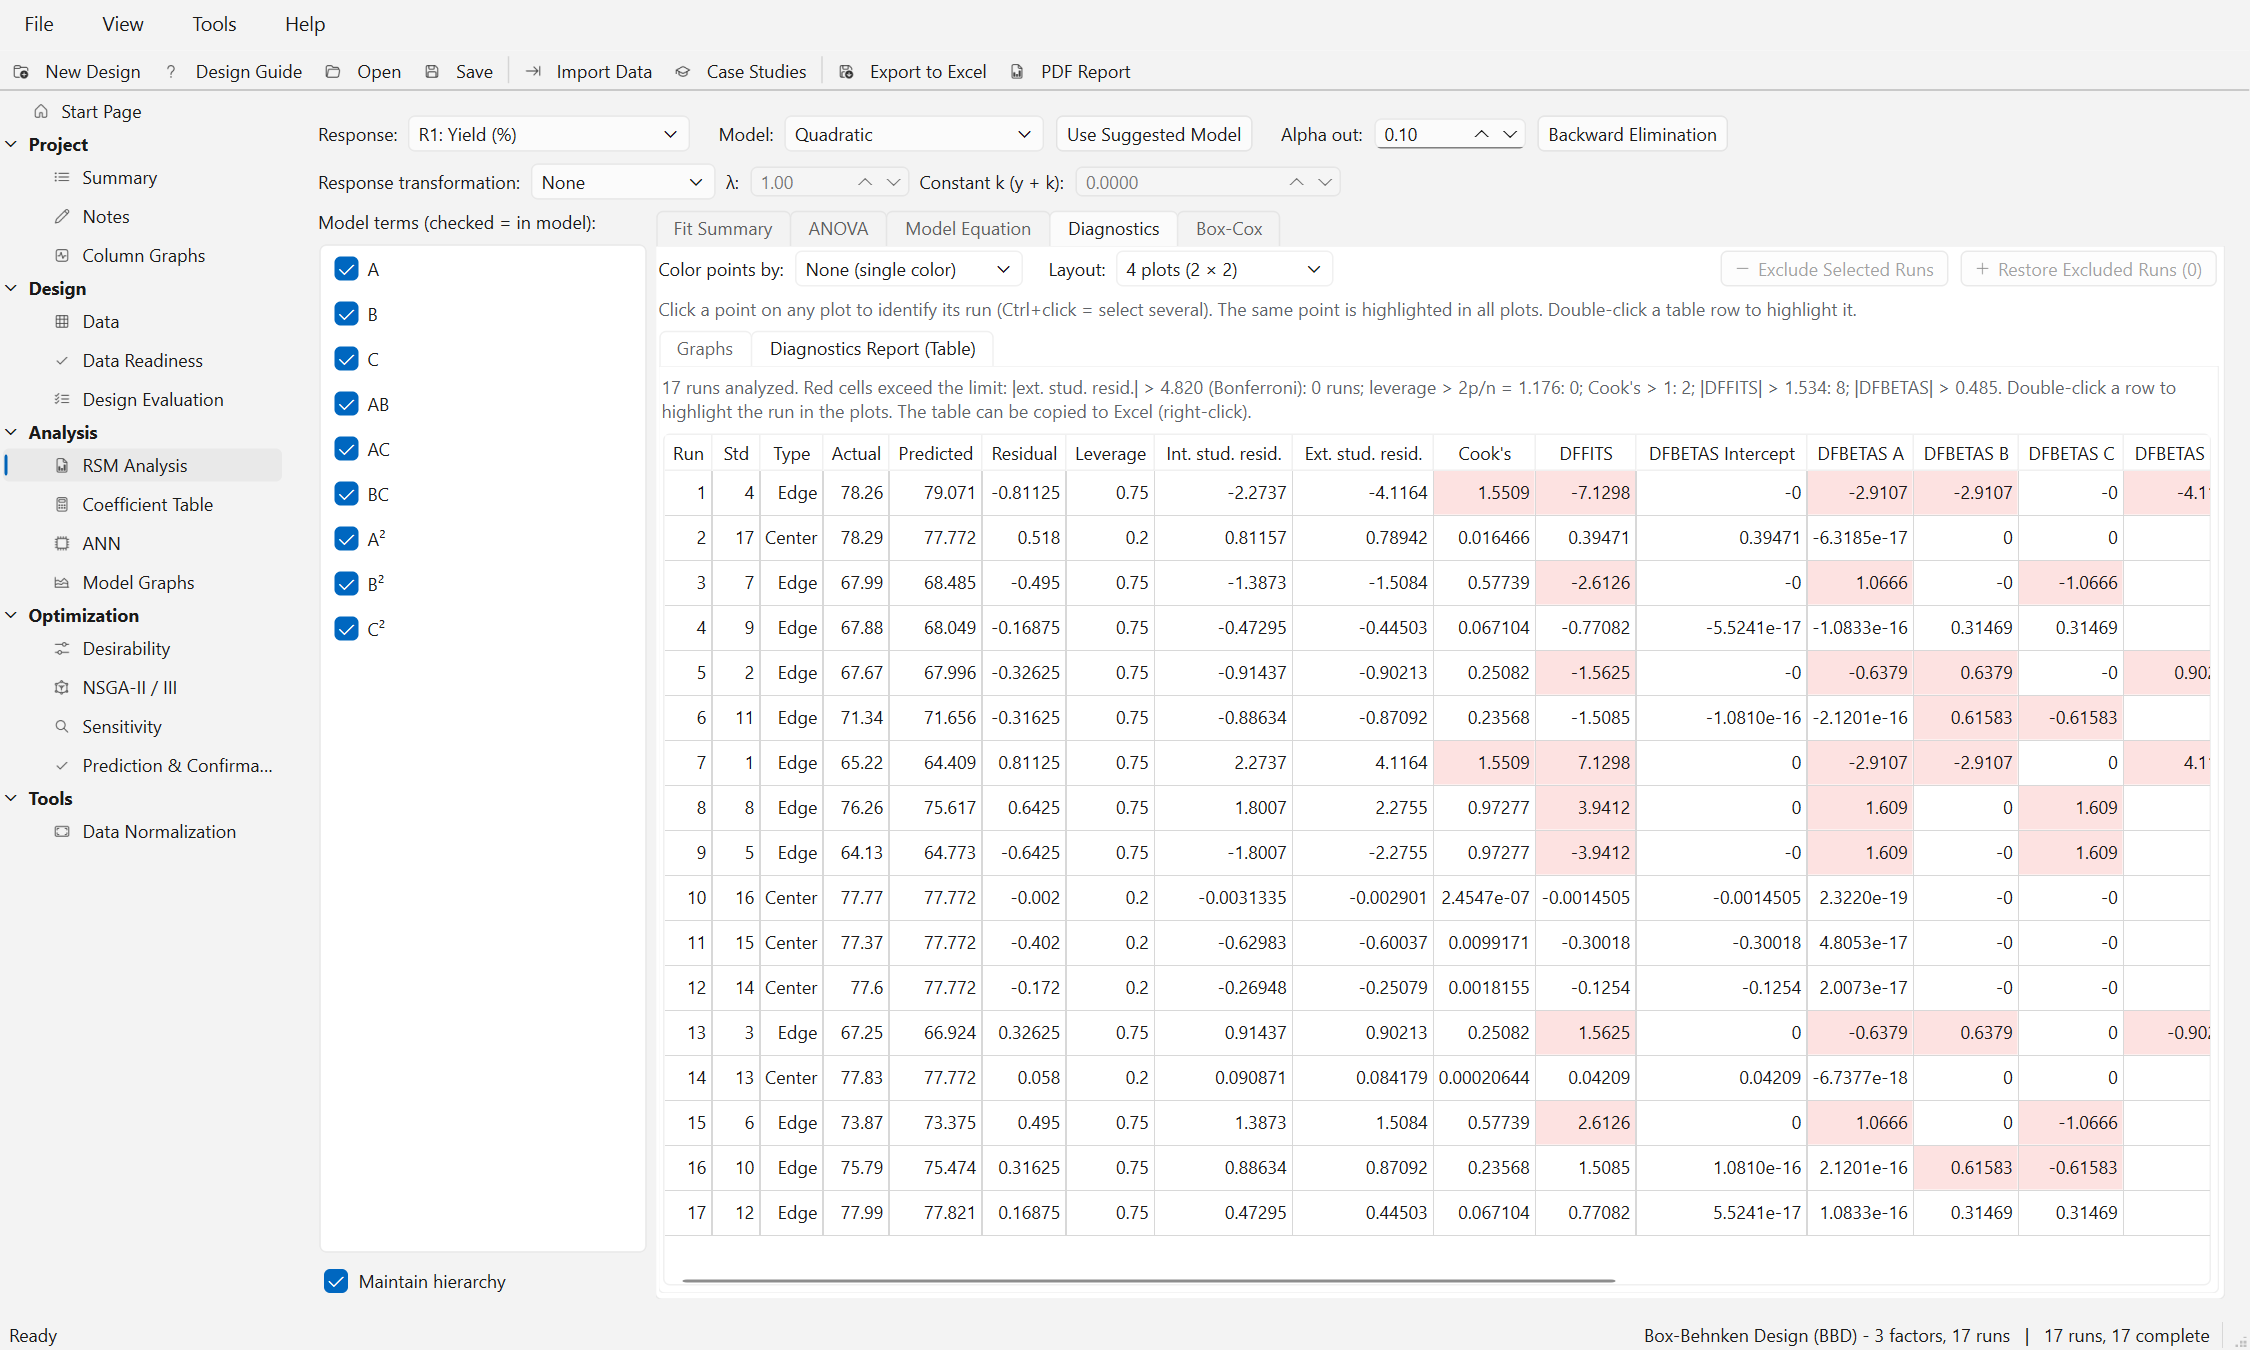
\includegraphics[width=\linewidth]{rsm_diagnostics_table.png}
\caption{Diagnostics Report (Table) for Yield (Box-Behnken case, no transformation) with the limits in the
header line (Cook's $>$ 1: 2 runs; $|$DFFITS$|$ $>$ 1.534: 8 runs) and red cells for values beyond them; all 17
runs are visible.}
\label{fig:ch05-diagtable}
\end{figure}

\subsection*{Excluding runs}
\ui{Exclude Selected Runs} (tooltip: ``Remove the runs from the analysis (the data is not deleted and can
be restored).'') marks the selected runs as excluded. Their response values are treated as missing by
every model, graph and optimization; the data stay on the \ui{Data} page and are marked in the Excel export
and the PDF report. \ui{Restore Excluded Runs (N)} brings all of them back. Exclude a run only when there is
a reason outside the statistics (a recorded mistake, a failed measurement), and always compare the model
before and after.

\subsection*{Example: Box-Behnken extraction, Yield}
Figures~\ref{fig:ch05-diag} and \ref{fig:ch05-diagtable} show the quadratic model. The normal plot is
close to a straight line and the Shapiro-Wilk $p$ is 0.904. The Bonferroni limit is
$t_{1-0.05/34,\,6}=4.820$; the largest $|t_i|$ is 4.12, so no run is an outlier. Leverage is 0.75 for the
edge runs and 0.20 for the center runs, all below $2p/n=1.176$. Runs 1 and 7 have Cook's distance 1.55
($>1$) and 8 runs exceed the DFFITS limit 1.534. Runs 1 and 7 are the AB-edge points (Temperature 60 °C,
Time 30 min) and (80 °C, 90 min). Excluding them shows why such a decision needs care: R² rises to 0.9973
and Predicted R² to 0.9675, but with only two AB-edge points left, AB and C² can no longer be separated and
C² is removed as aliased. The two runs carry the information about the AB interaction; they are influential
because the design has few runs, not because they are wrong. The Durbin-Watson statistic of this model is
1.98.

\section{Effects of two-level factorials}\label{sec:ch05-effects}

\subsection*{Purpose}
For unreplicated two-level designs there is no error estimate for a full model. The \ui{Effects (Factorial)}
sub-tab separates active effects from noise graphically and with Lenth's method \citep{lenth1989}.

\subsection*{When the sub-tab is shown}
The sub-tab appears for full factorial, fractional factorial and Plackett-Burman designs without categoric
factors and without split-plot structure. All numeric factor settings must be $-1$, 0 or $+1$ in coded
units (center points are allowed); otherwise the plot area shows ``Effect plots are only for 2-level
factorial designs.''

\subsection*{How to use}
\begin{enumerate}
  \item Choose the plot in \ui{Graph:} (\ui{Half-Normal}, \ui{Normal} or \ui{Pareto}).
  \item Click \ui{Select Automatically (Lenth ME Limit)}: every effect with $|\text{effect}|\ge\text{ME}$ is
        put in the model, together with its parent terms. If no effect qualifies: ``No effect exceeds the ME
        limit.''
  \item Click a point on the half-normal or normal plot (within 12 pixels) to add that term to the model or
        remove it; \ui{Maintain hierarchy} applies. Pareto bars are not clickable.
  \item \ui{Clear Selection} leaves the intercept-only model.
  \item Check the resulting model on the ANOVA sub-tab: the unselected effects now form the residual.
\end{enumerate}

\subsection*{Theory as implemented}
The program fits the model with all interactions of the factors (aliased columns removed) and computes each
effect as twice the coded coefficient, $c_j=2\hat\beta_j$, which is the difference between the mean response
at the high and at the low level. For Plackett-Burman designs only main effects are estimated, because
their two-factor interactions are partially aliased with the main effects; the unassigned columns then
provide residual degrees of freedom. With $m$ effects, Lenth's method is
\begin{align}
  s_0&=1.5\,\operatorname{median}_j|c_j|, \qquad
  \text{PSE}=1.5\,\operatorname{median}\{|c_j|:|c_j|<2.5\,s_0\}, \label{eq:ch05-pse}\\
  \text{ME}&=t_{0.975,\,d}\,\text{PSE},\qquad \text{SME}=t_{\gamma,\,d}\,\text{PSE},\qquad
  d=\frac m3,\quad \gamma=\frac{1+0.95^{1/m}}{2}. \label{eq:ch05-me}
\end{align}
PSE (pseudo standard error) is a robust estimate of the standard error of an effect based on the small
effects. ME is a margin of error for one effect at the 5\% level; SME is a simultaneous margin that controls
the error rate over all $m$ effects. An effect beyond SME is clearly active; one between ME and SME is
possibly active \citep{lenth1989}.

\paragraph{Plots.}
\begin{itemize}
  \item \emph{Half-Normal}: $|c_j|$ (axis \ui{|Effect|}) against the half-normal quantile of $(i-0.5)/m$
        (axis \ui{Half-normal (\%)}). Blue points are ``Error'', orange points ``Selected (model)''. Selected
        terms and terms beyond ME are labeled. A red dashed line through the origin follows the unselected
        effects (slope = median of $|c|/q$). Vertical lines show ``ME (Lenth)'' (dashed) and ``SME (Lenth)''
        (dotted).
  \item \emph{Normal}: signed effects (axis \ui{Effect}) against normal quantiles, with ME and SME on both
        sides.
  \item \emph{Pareto}: bars of $|t|$ sorted from large to small (orange = selected). Without residual df,
        $t=|c_j|/\text{PSE}$, the title adds ``(based on Lenth's PSE)'' and the lines are ME and SME in
        $t$ units ($t_{0.975,d}$ and $t_{\gamma,d}$). With residual df (replicates, center points or
        Plackett-Burman spare columns) $t=|c_j|/\text{se}(c_j)$ with lines ``t limit'' $t_{0.975,\nu}$
        and ``Bonferroni'' $t_{1-0.05/(2m),\nu}$.
\end{itemize}
The text below the plot gives ``PSE Lenth = \dots, ME = \dots, SME = \dots{} (Lenth 1989)'' and lists
aliased terms, if any.

\begin{figure}[htbp]\centering
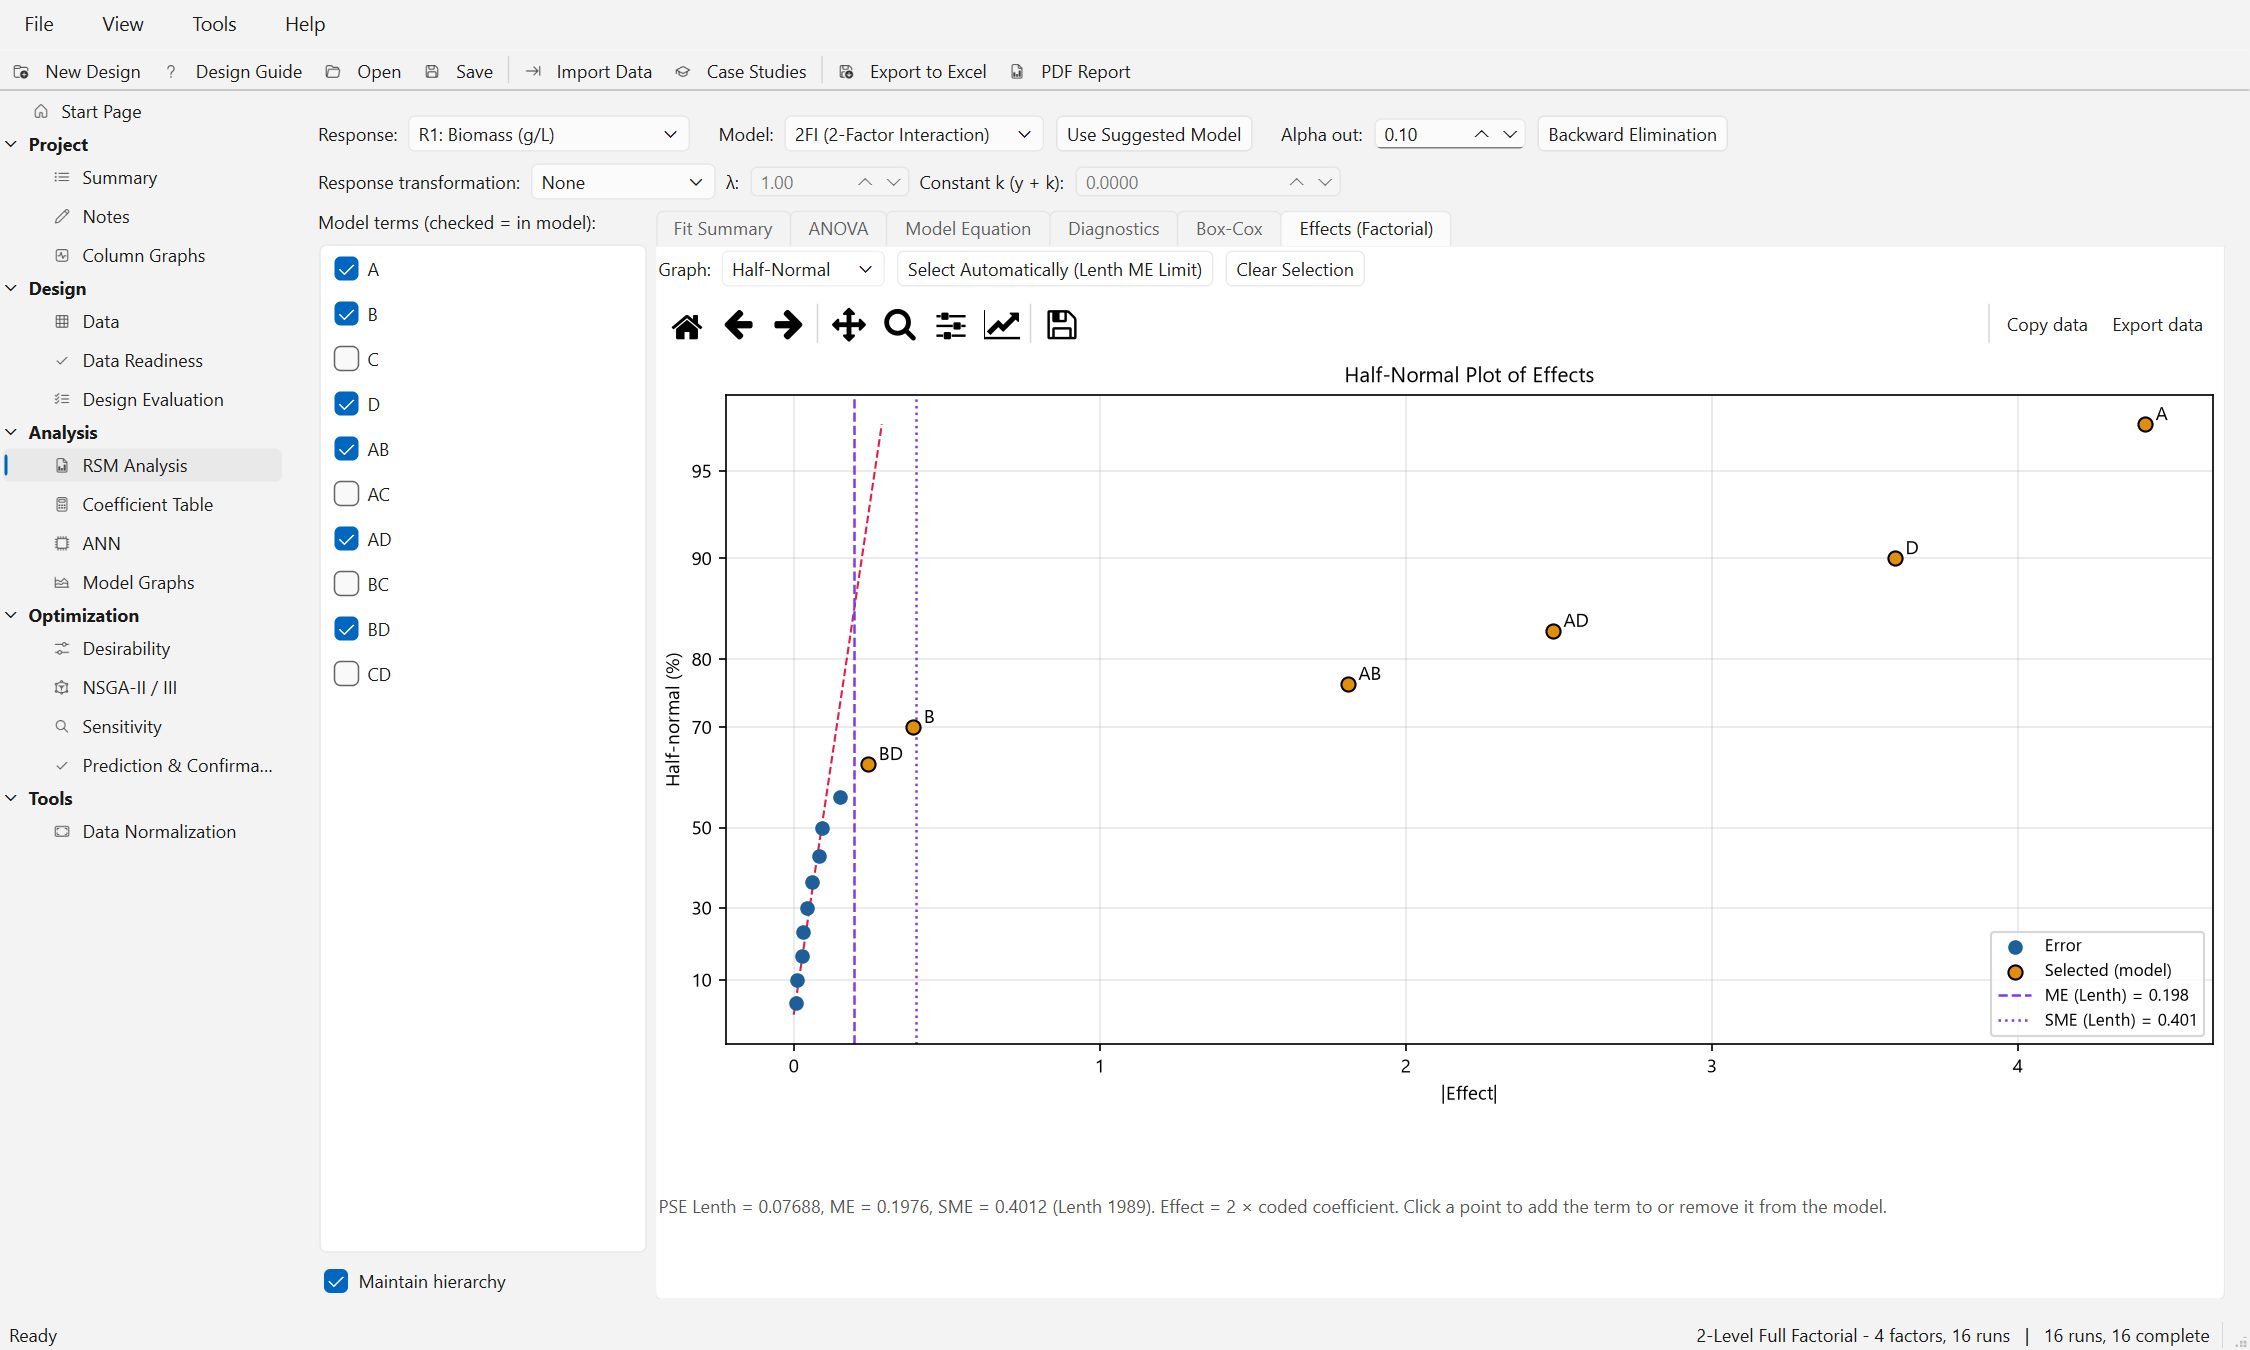
\includegraphics[width=\linewidth]{effects_halfnormal.png}
\caption{Half-normal plot of effects for Biomass (2$^4$ fermentation screening) after
\ui{Select Automatically (Lenth ME Limit)}, with the ME and SME lines.}
\label{fig:ch05-halfnormal}
\end{figure}

\begin{figure}[htbp]\centering
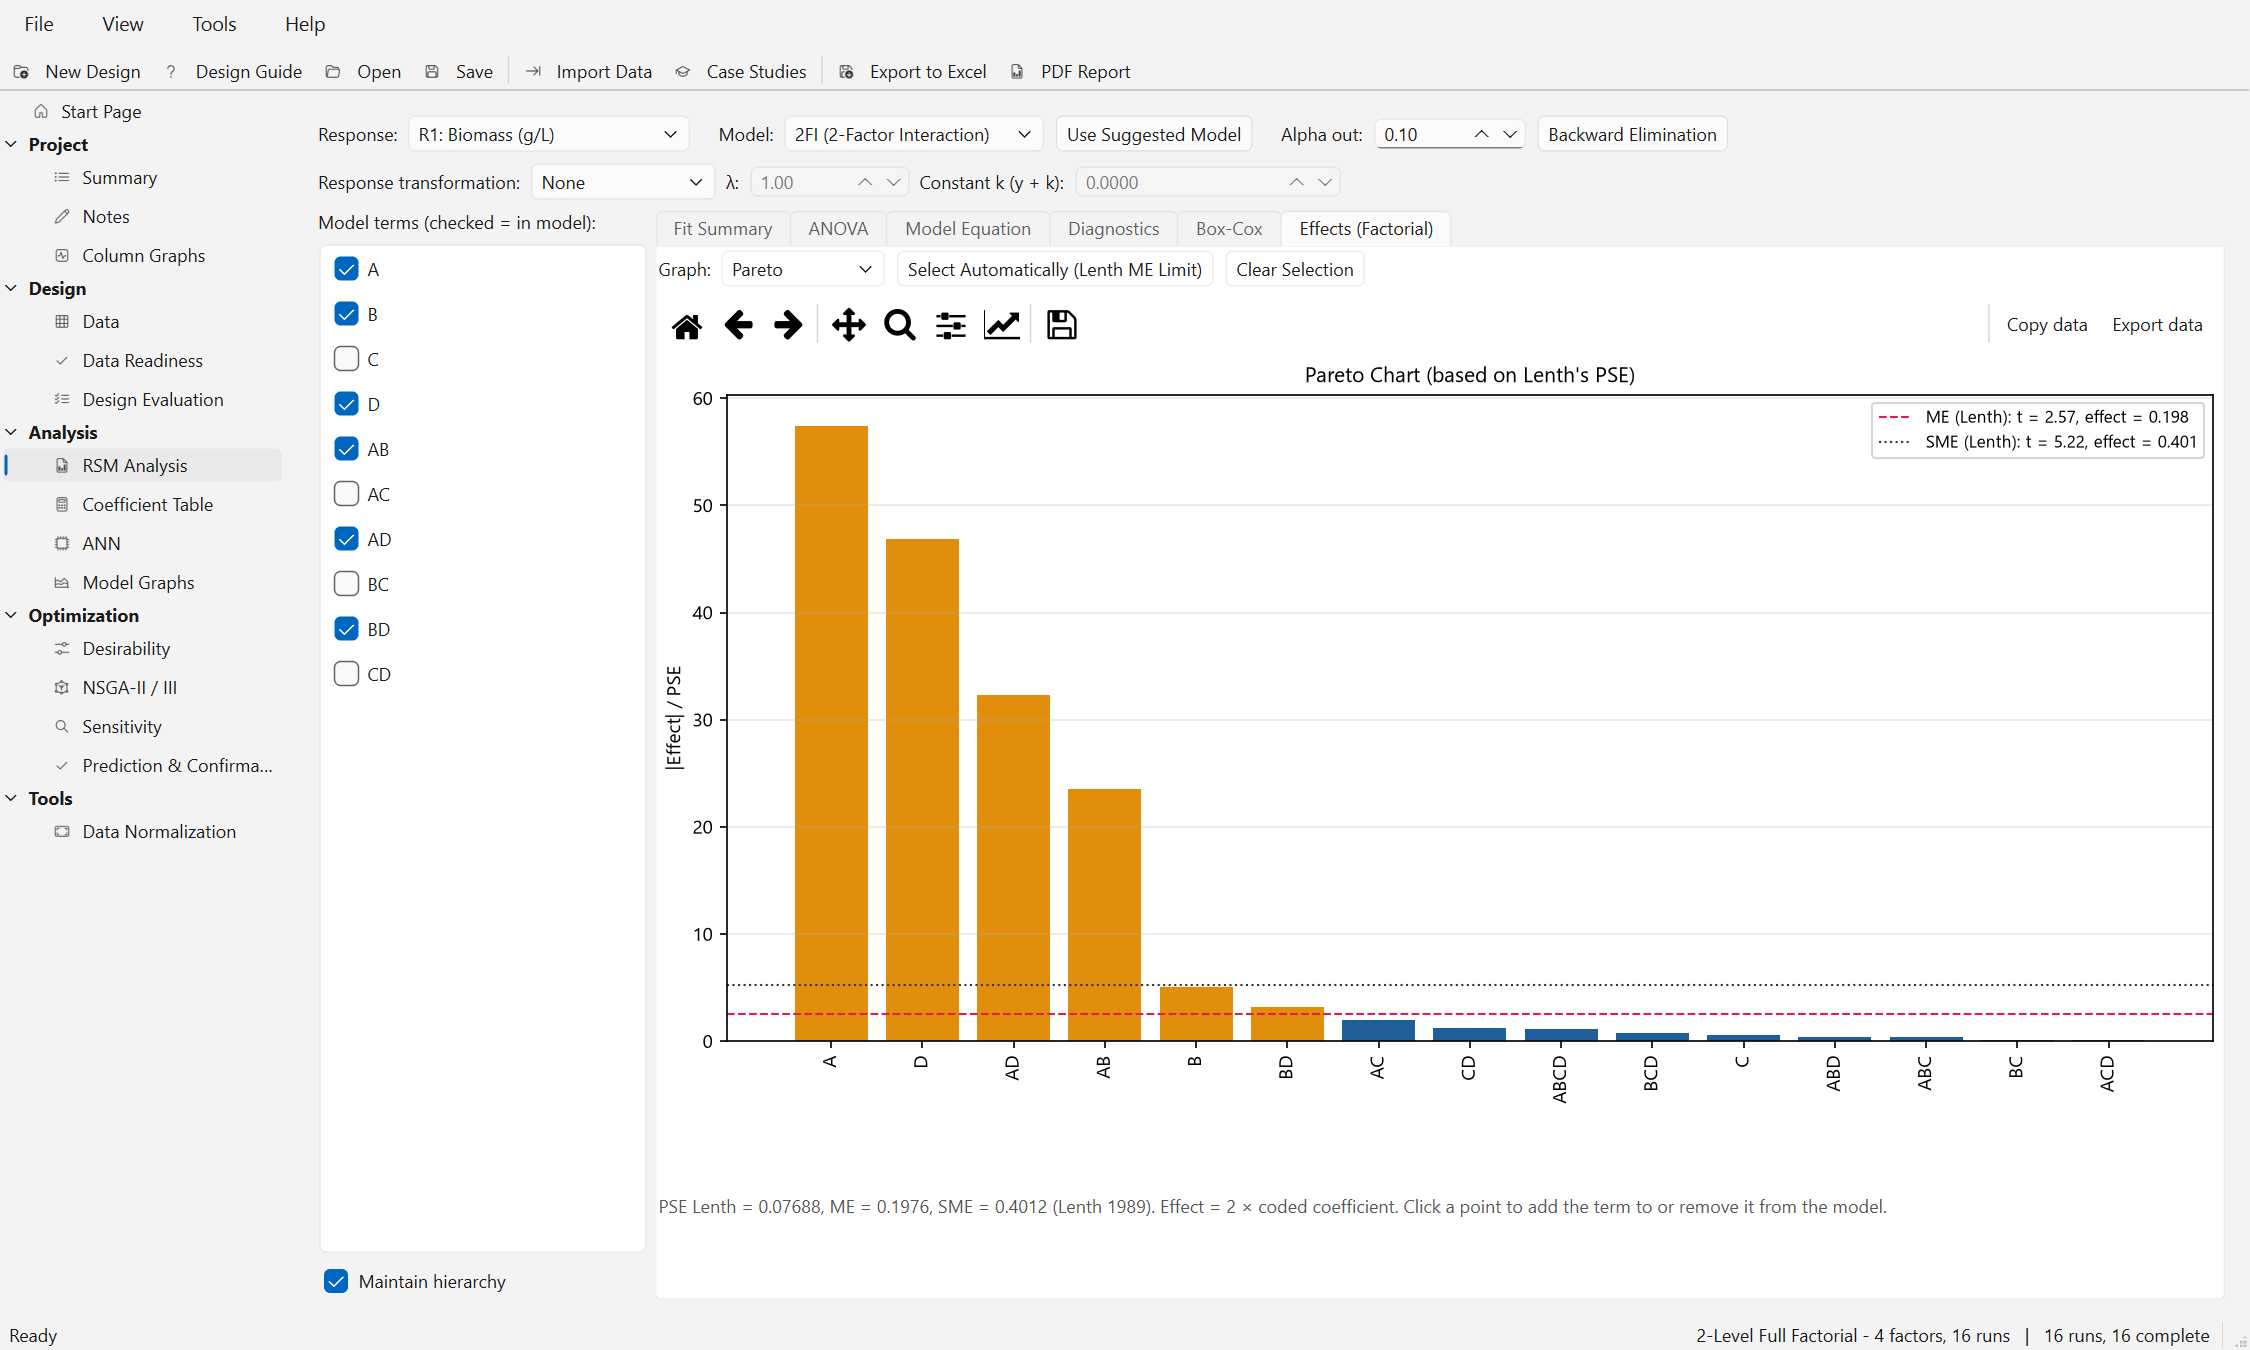
\includegraphics[width=\linewidth]{effects_pareto.png}
\caption{Pareto chart of the same effects, $|$effect$|$/PSE with the ME and SME limits.}
\label{fig:ch05-pareto}
\end{figure}

\subsection*{Example: Fermentation Screening (2$^4$ factorial)}
The 16 runs give 15 effects: A 4.416, D 3.599, AD 2.481, AB $-1.811$, B 0.391, BD $-0.244$; all others are
at most 0.151 in absolute value. Lenth's method gives PSE = 0.07688, ME = 0.1976 and SME = 0.4012
($d=5$, $t_{0.975,5}=2.571$, $t_{\gamma,5}=5.219$). \ui{Select Automatically (Lenth ME Limit)} selects A, B,
D, AB, AD and BD (Figure~\ref{fig:ch05-halfnormal}). A, D, AB and AD exceed SME; B and BD lie between ME and
SME, so they are only possibly active. The ANOVA of the selected model (Figure~\ref{fig:ch05-effanova}) has
9 residual df: Model $F=1385$ ($p<0.0001$), B $p=0.0004$, BD $p=0.0076$, R² 0.99892, Adjusted R² 0.9982,
Predicted R² 0.99658, Adeq Precision 107.0. The Fit Summary of this case (default 2FI) gives Linear
$p=0.0015$, 2FI $p<0.0001$ (Suggested) and 3FI $p=0.9165$; lack of fit cannot be tested because there are
no replicates.

\begin{figure}[htbp]\centering
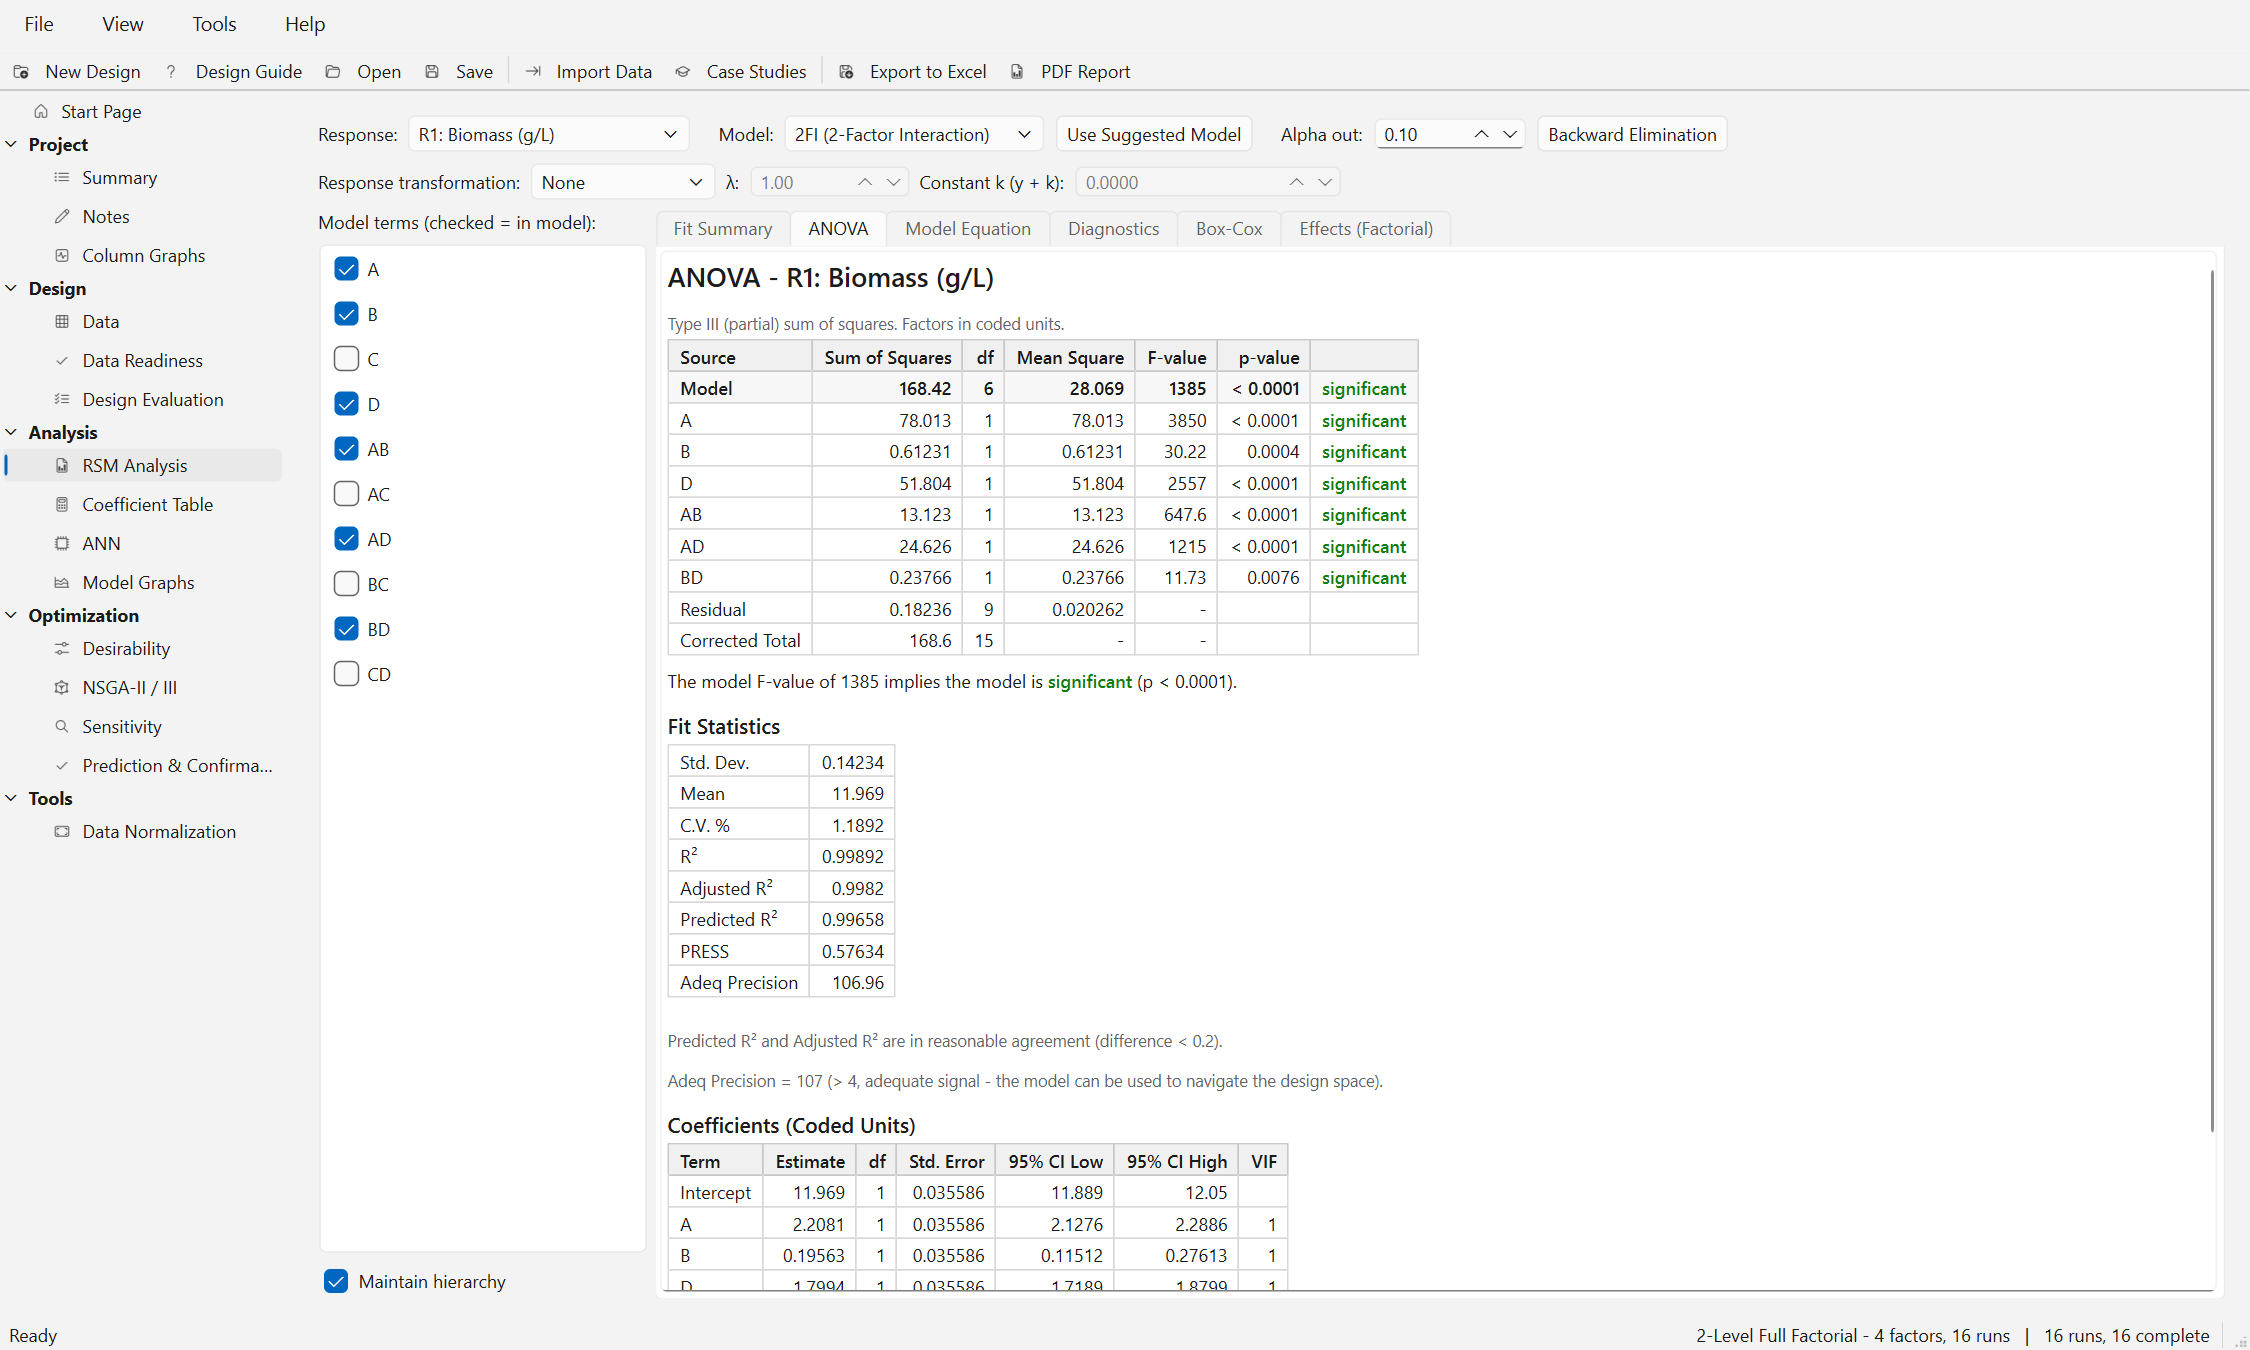
\includegraphics[width=\linewidth]{effects_anova.png}
\caption{ANOVA of the factorial model selected on the effects plot.}
\label{fig:ch05-effanova}
\end{figure}

\section{Logistic and Poisson regression (GLM)}\label{sec:ch05-glm}

\subsection*{Purpose}
Counts and numbers of successes do not have constant variance and cannot be negative or exceed the number
of trials. For such responses REGEN fits a generalized linear model (GLM) \citep{mccullagh1989} instead of
least squares.

\subsection*{How to use}
\begin{enumerate}
  \item On the \ui{Data} page click \ui{Factor \& Response Info\dots} and set \ui{Type} of the response to
        \ui{Binomial (successes out of n)} (enter \ui{Trials per run}) or \ui{Poisson (counts)}. Enter the
        data as the number of successes per run, or as counts.
  \item On the RSM Analysis page the ANOVA sub-tab is now called \ui{GLM (Logistic/Poisson)} and the
        transformation box is disabled.
  \item Choose the model with the Fit Summary (likelihood-ratio version), remove terms with
        \ui{Backward Elimination}, and check the diagnostics.
\end{enumerate}

\subsection*{Theory as implemented}
\paragraph{Model.} For run $i$ with $m$ trials and model row $x_i$:
\begin{align}
  \text{binomial:}\quad & y_i\sim\text{Bin}(m,\pi_i),\quad \ln\frac{\pi_i}{1-\pi_i}=x_i'\beta
  \quad\text{(logit link)}, \label{eq:ch05-logit}\\
  \text{Poisson:}\quad & y_i\sim\text{Pois}(\mu_i),\quad \ln\mu_i=x_i'\beta\quad\text{(log link)}.
  \label{eq:ch05-poisson}
\end{align}

\paragraph{Estimation (IRLS).} Starting from $\eta=\operatorname{logit}\bar p$,
$\bar p=(\sum y+0.5)/(mn+1)$ (binomial) or $\eta=\ln\max(y,0.5)$ (Poisson), the program iterates
\begin{equation}
  w_i=m\pi_i(1-\pi_i)\ \text{or}\ \mu_i,\qquad z_i=\eta_i+\frac{y_i-\mu_i}{w_i},\qquad
  \beta\leftarrow(X'WX)^{-1}X'Wz,
  \label{eq:ch05-irls}
\end{equation}
with $\mu_i=m\pi_i$ for the binomial, until $\max|\Delta\beta|<10^{-10}(1+\max|\beta|)$ or 100 iterations.
The covariance of $\hat\beta$ is $(X'WX)^{-1}$, so the Wald statistic is $z=\hat\beta_j/\text{se}_j$ and the
95\% CI uses 1.96.

\paragraph{Deviance and tests.} The deviance compares the model with the saturated model:
\begin{align}
  D_{\text{bin}}&=2\sum_i\Big[y_i\ln\frac{y_i}{\hat\mu_i}+(m-y_i)\ln\frac{m-y_i}{m-\hat\mu_i}\Big],
  \qquad D_{\text{Pois}}=2\sum_i\Big[y_i\ln\frac{y_i}{\hat\mu_i}-(y_i-\hat\mu_i)\Big]. \label{eq:ch05-dev}
\end{align}
The model is tested with $\chi^2=D_0-D$ on $p-p_0$ df, where the null model contains the intercept (and
blocks). Each term is tested by refitting without its columns: $\chi^2_t=D_{(-t)}-D$ on $df_t$ df (a
Type III likelihood-ratio test). The sequential test of the Fit Summary is $D_{\text{ref}}-D$ on
$p-p_{\text{ref}}$ df.

\paragraph{Goodness of fit and statistics.}
\begin{itemize}
  \item Deviance and Pearson $\chi^2=\sum(y_i-\hat\mu_i)^2/V(\hat\mu_i)$, with $V=\hat\mu(1-\hat\mu/m)$
        (binomial) or $V=\hat\mu$ (Poisson), are compared with $\chi^2_{n-p}$. Dispersion = Pearson
        $\chi^2/(n-p)$; values well above 1 mean overdispersion (the standard errors are then too small).
  \item Hosmer-Lemeshow test (binomial) \citep{hosmer1980}: the runs are sorted by $\hat\pi$ and split into
        $g=\min(10,\max(2,\lfloor n/2\rfloor))$ groups;
        $\chi^2_{HL}=\sum_g(O_g-E_g)^2/\big(N_g\bar\pi_g(1-\bar\pi_g)\big)$, with $O_g$, $E_g$ the observed
        and expected successes and $N_g$ the trials in group $g$, on $\max(g-2,1)$ df.
  \item AIC $=-2\ell+2p$, BIC $=-2\ell+p\ln n$, McFadden pseudo R² $=1-\ell/\ell_0$ and Adj.\ McFadden
        $=1-(\ell-p)/\ell_0$, where $\ell$ and $\ell_0$ are the log-likelihoods of the model and the null
        model.
  \item Tjur R² (binomial) \citep{tjur2009}: mean fitted probability of the successes minus that of the
        failures, $\sum y_i\hat\pi_i/\sum y_i-\sum(m-y_i)\hat\pi_i/\sum(m-y_i)$.
\end{itemize}

\paragraph{Warnings.} The program warns when IRLS does not converge within 100 iterations, and when fitted
probabilities are numerically 0 or 1 (binomial) or fitted means numerically 0 (Poisson). The latter
indicates complete or quasi-complete separation: some coefficients tend to infinity, and their standard
errors, $z$ tests and odds ratios are not reliable. Very large coefficients ($|\hat\beta|>10$) are then
listed. The warnings appear at the top of the GLM sub-tab, and the red error label says ``The GLM fit has
warnings - see the GLM (Logistic/Poisson) tab.'' Remove terms or add runs where the response changes.

\paragraph{Diagnostics and predictions.} Residuals are deviance residuals
$\text{sign}(y_i-\hat\mu_i)\sqrt{d_i}$ standardized by $\sqrt{1-h_{ii}}$, with leverage from $W^{1/2}X$.
Cook's distance is $r_{P,i}^2h_{ii}/\big(p(1-h_{ii})^2\big)$ with the Pearson residual $r_{P,i}$; DFFITS uses
the standardized deviance residual; DFBETAS is not available. \ui{Predicted vs Actual} is on the response
scale: observed proportion against fitted probability, or observed count against fitted mean. Predictions,
graphs and optimization use $\hat\pi$ or $\hat\mu$; the 95\% CI is $g^{-1}(\hat\eta\pm1.96\,\text{se}_\eta)$.
No prediction interval is given.

\subsection*{Output}
The sub-tab (Figure~\ref{fig:ch05-glm}) shows the heading ``Logistic Regression - \dots'' or ``Poisson
Regression - \dots'', the note ``Link: logit. Trials per run = 50. Terms are tested with the likelihood ratio
($\chi^2$).'', the test table (\ui{Source}, \ui{$\chi^2$}, \ui{df}, \ui{p-value}), \ui{Fit Statistics},
\ui{Goodness-of-Fit Tests} and the coefficient table on the logit or log scale with \ui{z}, \ui{p-value},
confidence limits and \ui{Odds ratio} or \ui{Rate ratio} $=e^{\hat\beta}$. The note under the GOF table
reads: ``A goodness-of-fit p-value $>$ 0.05 means there is no evidence of lack of fit. Dispersion well
above 1 indicates overdispersion.''

\begin{figure}[htbp]\centering
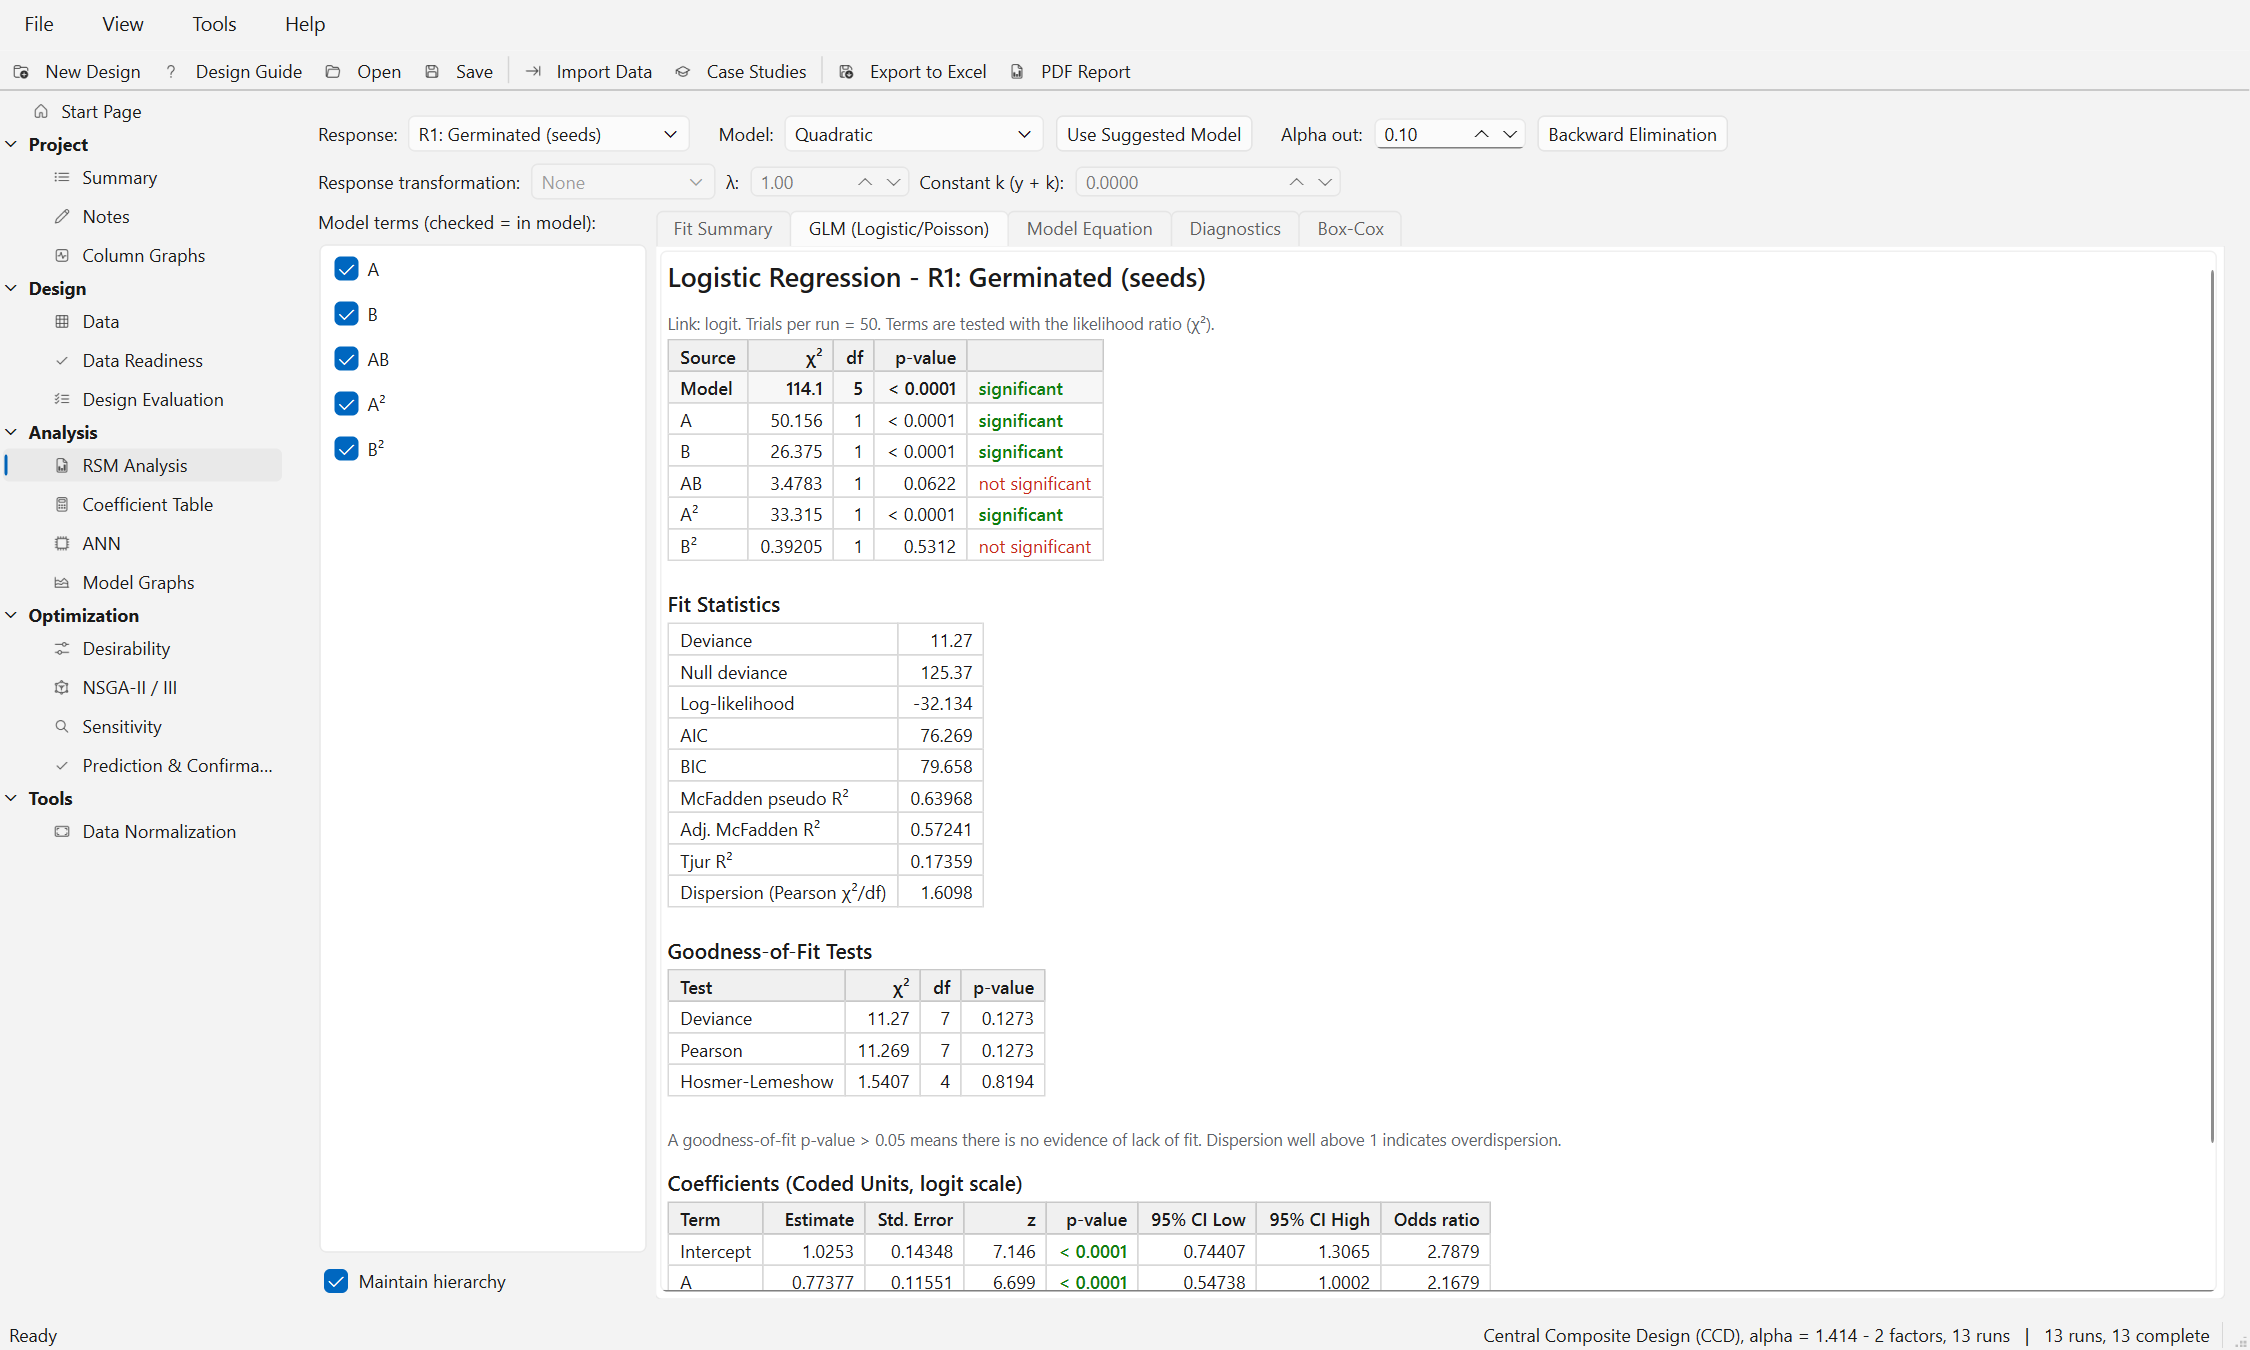
\includegraphics[width=\linewidth]{glm_logistic.png}
\caption{GLM (Logistic/Poisson) sub-tab for the seed germination case: likelihood-ratio tests, fit
statistics, goodness-of-fit tests and coefficients with odds ratios.}
\label{fig:ch05-glm}
\end{figure}

\subsection*{Example: Seed Germination (logistic regression)}
The case is a CCD in Temperature (20--35 °C) and Humidity (60--90\%) with 13 runs of 50 seeds. The Fit
Summary gives Linear ($p<0.0001$, deviance 46.94, AIC 105.94), 2FI ($p=0.1257$), Quadratic ($p<0.0001$,
deviance 11.27, AIC 76.27, McFadden 0.640, Suggested) and Cubic ($p=0.384$, Aliased). For the quadratic
model the likelihood-ratio tests are: Model $\chi^2=114.1$ on 5 df, A 50.16, B 26.38, AB 3.48 ($p=0.0622$),
A² 33.32 and B² 0.39 ($p=0.5312$). Deviance 11.27 on 7 df ($p=0.1273$), Pearson $p=0.1273$,
Hosmer-Lemeshow $\chi^2=1.54$ on 4 df ($p=0.8194$): no lack of fit. Dispersion is 1.61, slightly above 1.
McFadden R² is 0.640 (adjusted 0.572), Tjur R² 0.174. Tjur's R² is small because it measures how well single
seeds are separated, and the germination probability only ranges over moderate values. The odds ratios
are A 2.168, B 1.777, AB 0.742 and A² 0.495. Because the model contains AB and A², an odds ratio of a
single coefficient is not the change in odds for a change of the factor; use the model graphs to see the
combined effect. IRLS converged in 5 iterations without warnings. At the center the
predicted germination probability is 0.736 (95\% CI 0.678 to 0.787).

\section{Split-plot analysis with REML}\label{sec:ch05-reml}

\subsection*{Purpose}
In a split-plot experiment the hard-to-change (HTC) factors are set once per whole plot, and the
easy-to-change factors vary within it. Runs in the same whole plot share a random whole-plot error, so
ordinary least squares gives wrong tests: HTC effects look more significant than they are. REGEN fits a
linear mixed model by restricted maximum likelihood (REML) \citep{patterson1971,goos2011}.

\subsection*{How to use}
The analysis is used automatically for projects with whole plots (created with the split-plot option in
\ui{New Design}, with the hard-to-change factor letters). The ANOVA sub-tab is called
\ui{Split-Plot (REML)}, \ui{Use Suggested Model} is hidden, the Fit Summary is not available and Box-Cox is
not offered. Transformations, term selection and backward elimination work as usual. There is no overall
model F test and no least-squares R², adjusted R² or predicted R² for this model (only the conditional R² of
the statistics table); judge it by the Wald F tests of its terms. The
\ui{Data Readiness} page therefore shows ``Model fit'' and ``Model significance'' as Info checks for split-plot
responses (Chapter~\ref{chap:4}).

\subsection*{Theory as implemented}
\paragraph{Model.}
\begin{equation}
  y=X\beta+Zu+\varepsilon,\qquad u_g\sim N(0,\sigma^2_{wp}),\quad \varepsilon_i\sim N(0,\sigma^2),
  \label{eq:ch05-mixed}
\end{equation}
where $Z$ assigns runs to whole plots. With $\gamma=\sigma^2_{wp}/\sigma^2$ the covariance is
$\sigma^2V_0$, $V_0=I+\gamma ZZ'$. Each whole-plot block of $V_0^{-1}$ is
$I-\frac{\gamma}{1+\gamma m_g}J$ ($m_g$ runs in plot $g$, $J$ a matrix of ones) and
$\ln|V_0|=\sum_g\ln(1+\gamma m_g)$.

\paragraph{REML.} For a given $\gamma$, the generalized least-squares estimate and the profile REML criterion
are
\begin{align}
  \hat\beta&=(X'V_0^{-1}X)^{-1}X'V_0^{-1}y,\qquad
  \hat\sigma^2=\frac{r'V_0^{-1}r}{n-p},\quad r=y-X\hat\beta, \label{eq:ch05-gls}\\
  -2\ell_R(\gamma)&=(n-p)\ln\hat\sigma^2+\ln|V_0|+\ln|X'V_0^{-1}X| \quad(\text{constants omitted}).
  \label{eq:ch05-reml}
\end{align}
The criterion is minimized over $\ln\gamma\in[-12,9]$. If the value at $\ln\gamma=-30$ is not worse, the
whole-plot variance is set to 0 (boundary). Then $\hat\sigma^2_{wp}=\gamma\hat\sigma^2$ and
$\text{Cov}(\hat\beta)=\hat\sigma^2(X'V_0^{-1}X)^{-1}$.

\paragraph{Wald F tests and denominator df.} Each term $t$ with $q_t$ columns is tested with
$F=\hat\beta_t'C_t^{-1}\hat\beta_t/q_t$, where $C_t$ is its block of $\text{Cov}(\hat\beta)$. The denominator
df follow the containment rule:
\begin{align}
  df_{wp}&=n_{wp}-(1+c_{wp}),\qquad df_{sp}=n-n_{wp}-(p-1-c_{wp}), \label{eq:ch05-dfcont}
\end{align}
with $n_{wp}$ whole plots and $c_{wp}$ the number of columns of whole-plot terms (terms made only of HTC
factors). The intercept and whole-plot terms are tested on $df_{wp}$, all other terms on $df_{sp}$. If a df
is 0, $n-p$ is used instead. The coefficient $t$ tests use the same df. The more refined Kenward-Roger
correction \citep{kenward1997} is not implemented; with few whole plots its df can be smaller.

\paragraph{Residuals.} The whole-plot effects are predicted by
$\hat u_g=\frac{\gamma}{1+\gamma m_g}\sum_{i\in g}r_i$ (BLUP). Diagnostics use the conditional residuals
$r_i-\hat u_{g(i)}$, studentized by $\sqrt{\hat\sigma^2(1-h_i/(1+\gamma))}$ with
$h_i=x_i'(X'V_0^{-1}X)^{-1}x_i$. Conditional R² $=1-\sum(r_i-\hat u_{g(i)})^2/\text{SST}$. Cook's distance and
DFFITS are not shown (neither in the plots nor in the table): their one-run deletion formulas assume
independent runs, which is not true within a whole plot, and a proper deletion diagnostic would have to
re-estimate the variance components. DFBETAS is not available either.

\paragraph{Predictions.} The confidence interval uses $\text{Cov}(\hat\beta)$; the prediction interval
for the mean of $m$ new runs adds $\hat\sigma^2_{wp}+\hat\sigma^2/m$. The POE graph uses
$\hat\sigma^2+\hat\sigma^2_{wp}$ as residual variance.

\subsection*{Output}
The sub-tab (Figure~\ref{fig:ch05-reml}) shows the heading ``Split-Plot Analysis (REML) - \dots'', the
note on the containment method, the test table (\ui{Term}, \ui{Type} = Whole plot or Subplot,
\ui{Numerator df}, \ui{Denominator df}, \ui{F-value}, \ui{p-value}), \ui{Variance Components} (\ui{Whole plot
(between groups)} and \ui{Subplot (residual)} with variance, standard deviation and \% of the total),
\ui{Statistics} (number of whole plots, df whole plot, df subplot, variance ratio $\gamma$, $-2$ REML
log-likelihood, conditional R², mean) and \ui{Coefficients (GLS)} with $t$ tests. If $df_{wp}\le0$ the
warning ``Whole-plot df = 0: hard-to-change factor effects cannot be tested properly. Add more whole plots
(replicates).'' is shown.

\begin{figure}[htbp]\centering
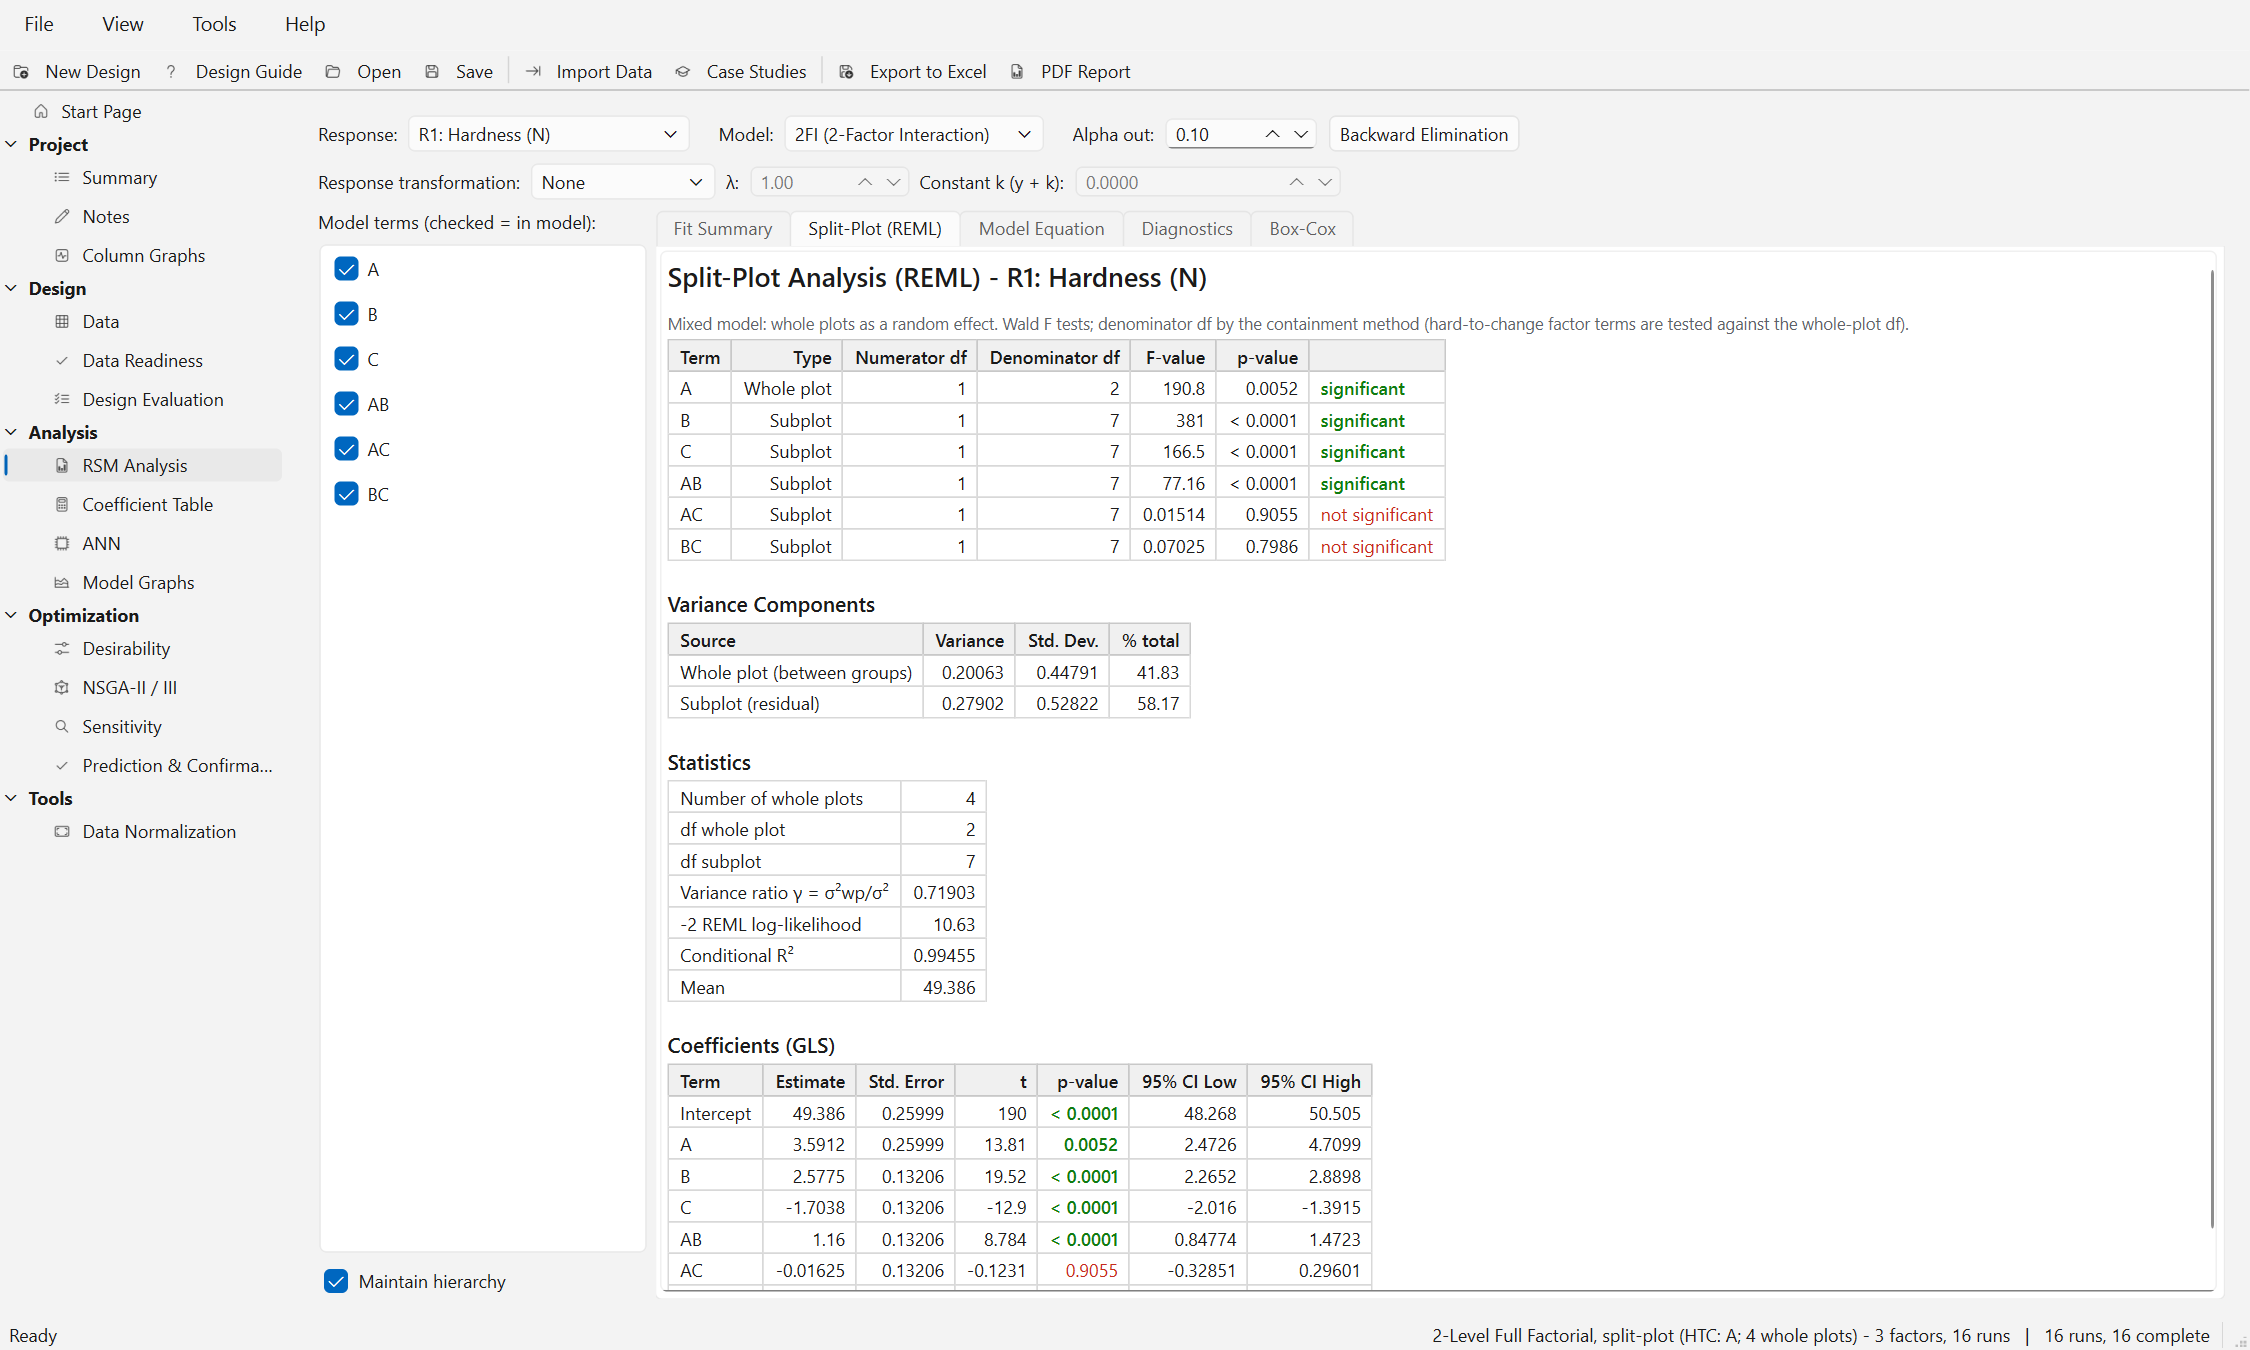
\includegraphics[width=\linewidth]{reml_splitplot.png}
\caption{Split-Plot (REML) sub-tab for the oven hardness case: Wald F tests with whole-plot and subplot
denominator df, variance components and statistics.}
\label{fig:ch05-reml}
\end{figure}

\subsection*{Example: Oven Product Hardness (split-plot)}
Oven Temperature (A) is hard to change; Time (B) and Concentration (C) are easy to change. The $2^3$ design
is replicated twice (16 runs) in 4 whole plots of 4 runs. For the default 2FI model ($p=7$),
\eqref{eq:ch05-dfcont} gives $df_{wp}=4-(1+1)=2$ and $df_{sp}=16-4-(7-1-1)=7$. Results: A (whole plot)
$F=190.8$ on 1 and 2 df, $p=0.0052$; B $F=381.0$, C $F=166.5$, AB $F=77.2$ (subplot, 7 df, all
$p<0.0001$); AC $p=0.9055$ and BC $p=0.7986$. The variance components are $\hat\sigma^2_{wp}=0.2006$
(41.8\%) and $\hat\sigma^2=0.2790$ (58.2\%), $\gamma=0.719$, $-2\ell_R=10.63$, conditional R² 0.99455. Although
A has the largest $F$ after B, its p-value is the largest of the active terms because it is judged against
only 2 df: the experiment has just 4 independent oven settings. Backward elimination at 0.10 removes AC and
BC.

\section{Coefficient Table page}\label{sec:ch05-coeftable}

\subsection*{Purpose}
The \ui{Coefficient Table} page (navigation group \ui{Analysis}) shows the coded coefficients of all
responses side by side, so you can see at a glance which factor affects which response and in which
direction.

\subsection*{How to use}
Open the page; it always reflects the current model of each response. The only option is the check box
\ui{Show p-values} (default on), which prints the p-value under each coefficient.

\subsection*{Output and how to read it}
\begin{itemize}
  \item Heading ``Coefficient Table (coded factors)''; one row per coefficient label (all responses
        together) and one column per response that has a model. An empty cell means that the term is not in
        that response's model.
  \item Cell color by the p-value of the coefficient: $p<0.01$ green, $p<0.05$ light green, $p<0.10$
        yellow; the intercept is never colored. The p-values are two-sided $t$ tests on $n-p$ df for least
        squares, Wald $z$ tests for GLM responses and $t$ tests with the containment df for REML responses
        (Section~\ref{sec:ch05-reml}).
  \item Footer rows: \ui{Transform}, \ui{Model} (order), \ui{p model} (model F test or GLM
        likelihood-ratio test; a dash for REML), \ui{R²} (McFadden R² for GLM, conditional R² for REML),
        \ui{Adj R²}, \ui{Pred R²} and \ui{Used for optimization} (\ui{RSM} or \ui{ANN} with its
        architecture).
  \item Closing note: coefficients are in coded units, so their sizes can be compared across factors; for
        responses that use an ANN the table still shows the RSM coefficients.
\end{itemize}
Because the factors are coded $-1$ to $+1$, a coefficient is half the change of the response from the low
to the high level of that factor (other factors at the center). Signs show conflicts between responses.

\begin{figure}[htbp]\centering
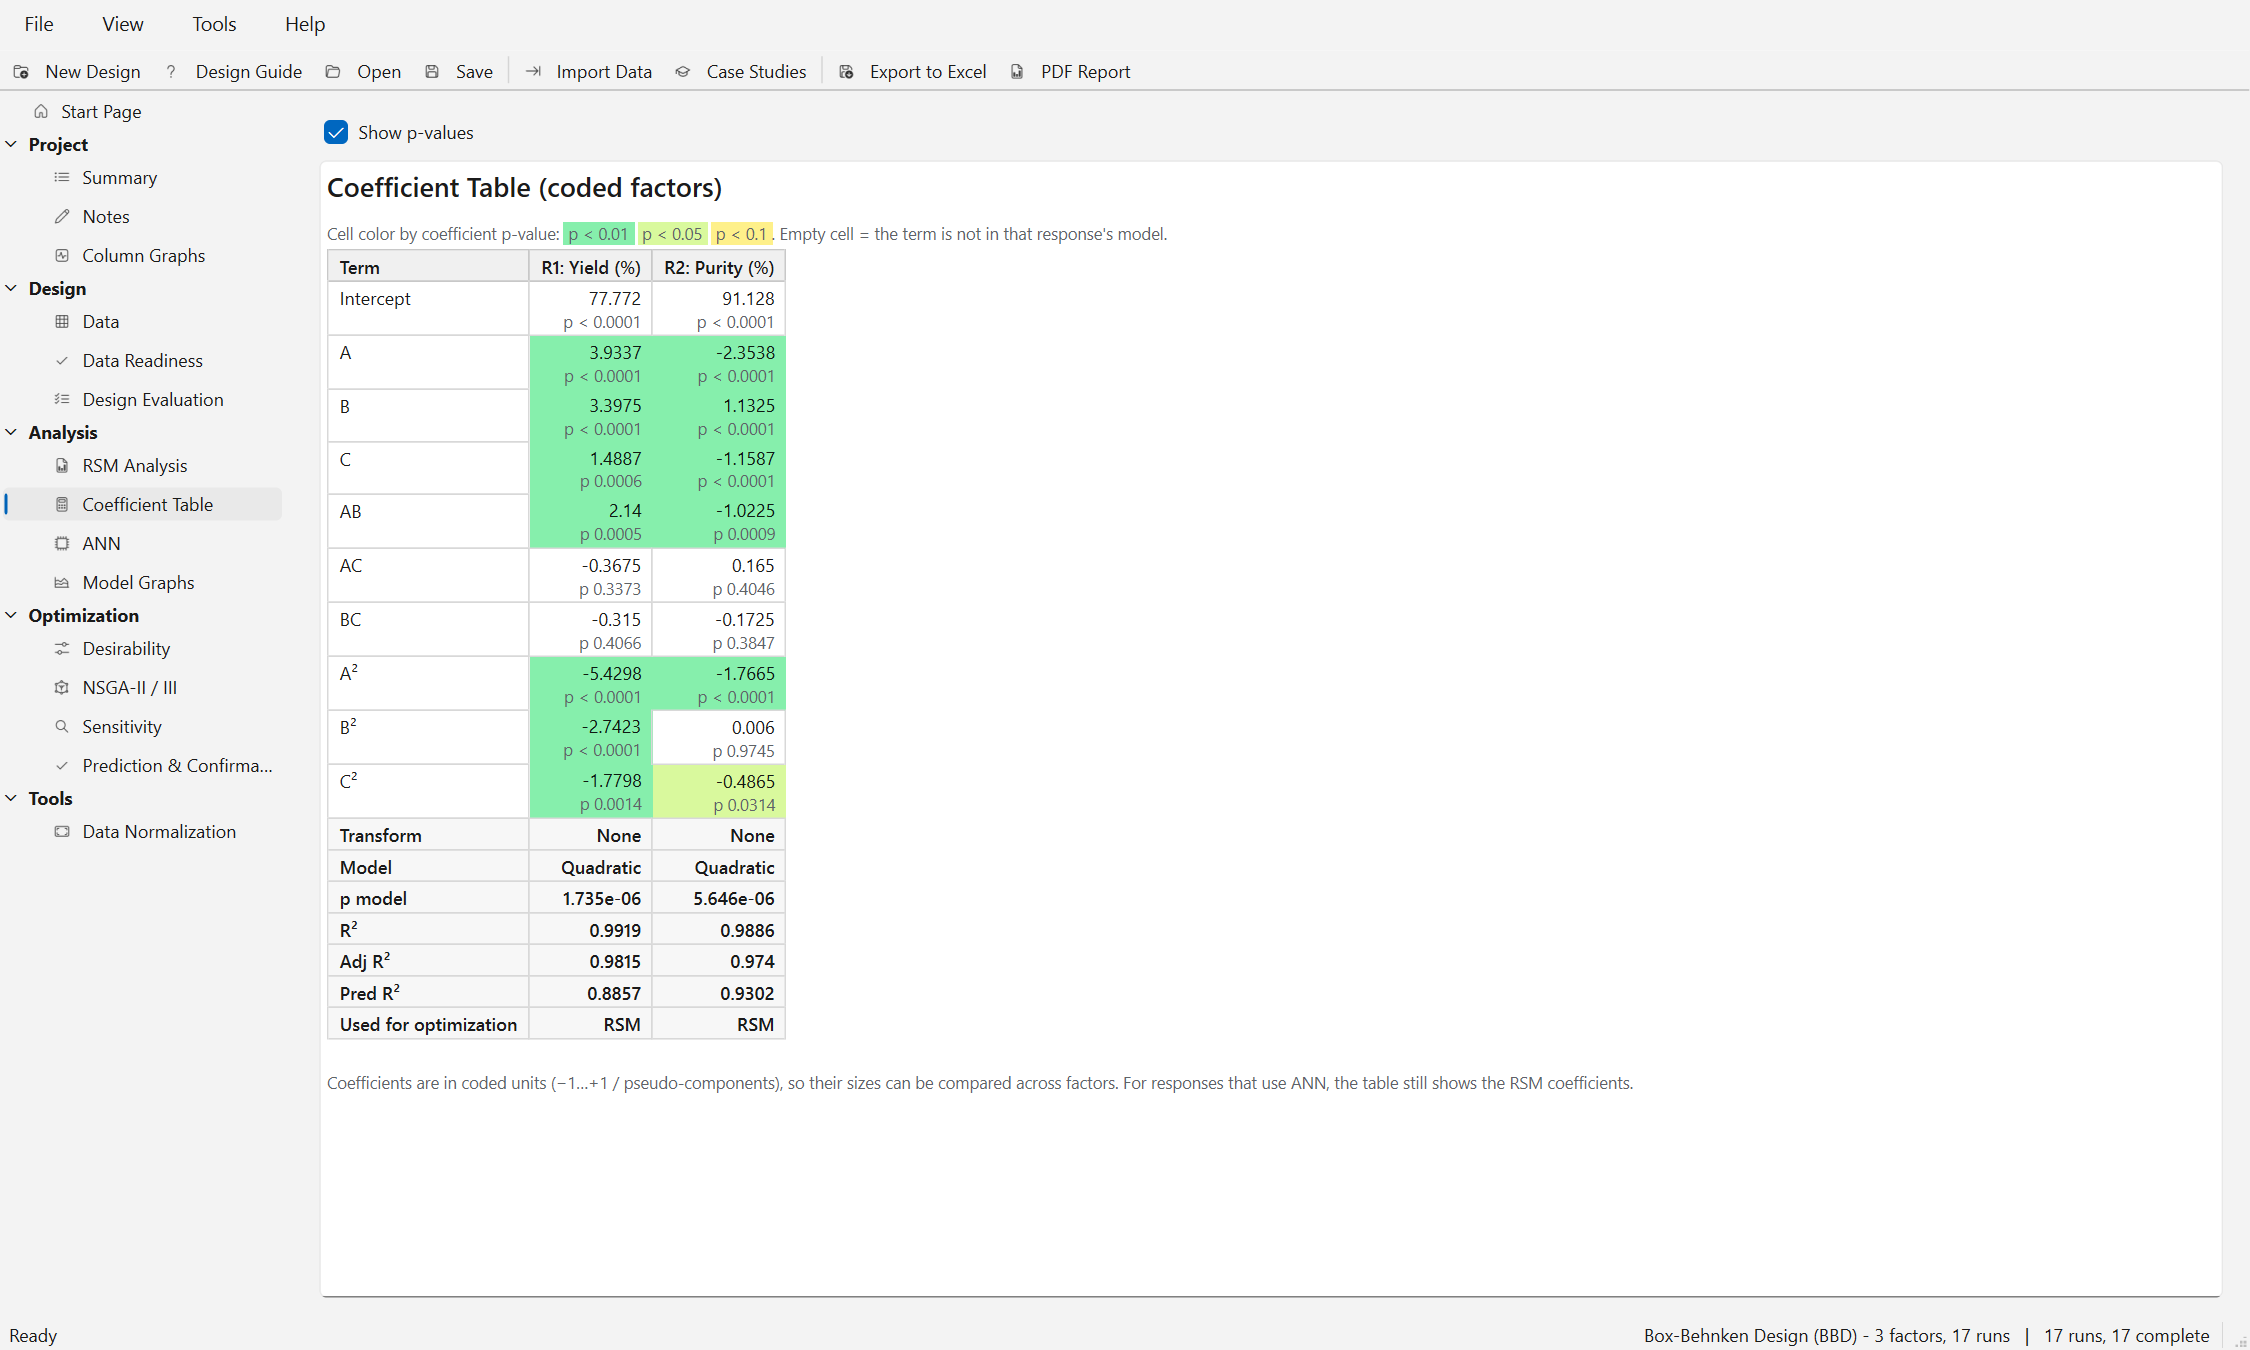
\includegraphics[width=\linewidth]{coefficient_table.png}
\caption{Coefficient Table for the Box-Behnken extraction case (Yield and Purity) with p-values and
p-value colors.}
\label{fig:ch05-coeftable}
\end{figure}

\subsection*{Example}
For the Box-Behnken case (Figure~\ref{fig:ch05-coeftable}) Temperature raises Yield ($A=3.9337$) but lowers
Purity ($A=-2.3538$), while Time raises both ($B=3.3975$ and 1.1325). The curvature in Temperature is strong
for both responses ($A^2=-5.4298$ and $-1.7665$). AC and BC are uncolored for both responses (p 0.34 to 0.41),
and B² of Purity ($p=0.9745$) is a candidate for removal. The conflict in Temperature is the reason why the
two responses must be optimized together (desirability or NSGA-II).

\subsection*{Data export}
Right-click the table for \ui{Copy all tables (for Excel)} or \ui{Export all tables\dots}. The PDF report
includes this table when the project has more than one response.
